\documentclass{article}

% packages
  % basic stuff for rendering math
  \usepackage[letterpaper, top=1in, bottom=1in, left=1in, right=1in]{geometry}
  \usepackage[utf8]{inputenc}
  \usepackage[english]{babel}
  \usepackage{amsmath} 
  \usepackage{amssymb}
  % \usepackage{amsthm}

  % extra math symbols and utilities
  \usepackage{mathtools}        % for extra stuff like \coloneqq
  \usepackage{mathrsfs}         % for extra stuff like \mathsrc{}
  \usepackage{centernot}        % for the centernot arrow 
  \usepackage{bm}               % for better boldsymbol/mathbf 
  \usepackage{enumitem}         % better control over enumerate, enumerate
  \usepackage{hyperref}         % for hypertext linking
  \usepackage{fancyvrb}          % for better verbatim environments
  \usepackage{newverbs}         % for texttt{}
  \usepackage{xcolor}           % for colored text 
  \usepackage{listings}         % to include code
  \usepackage{lstautogobble}    % helper package for code
  \usepackage{parcolumns}       % for side by side columns for two column code
  

  % page layout
  \usepackage{fancyhdr}         % for headers and footers 
  \usepackage{lastpage}         % to include last page number in footer 
  \usepackage{parskip}          % for no indentation and space between paragraphs    
  \usepackage[T1]{fontenc}      % to include \textbackslash
  \usepackage{footnote}
  \usepackage{etoolbox}

  % for custom environments
  \usepackage{tcolorbox}        % for better colored boxes in custom environments
  \tcbuselibrary{breakable}     % to allow tcolorboxes to break across pages

  % figures
  \usepackage{pgfplots}
  \pgfplotsset{compat=1.18}
  \usepackage{float}            % for [H] figure placement
  \usepackage{tikz}
  \usepackage{tikz-cd}
  \usepackage{circuitikz}
  \usetikzlibrary{arrows}
  \usetikzlibrary{positioning}
  \usetikzlibrary{calc}
  \usepackage{graphicx}
  \usepackage{caption} 
  \usepackage{subcaption}
  \captionsetup{font=small}

  % for tabular stuff 
  \usepackage{dcolumn}

  \usepackage[nottoc]{tocbibind}
  \pdfsuppresswarningpagegroup=1
  \hfuzz=5.002pt                % ignore overfull hbox badness warnings below this limit

% New and replaced operators
  \DeclareMathOperator{\Tr}{Tr}
  \DeclareMathOperator{\Sym}{Sym}
  \DeclareMathOperator{\Span}{span}
  \DeclareMathOperator{\std}{std}
  \DeclareMathOperator{\Cov}{Cov}
  \DeclareMathOperator{\Var}{Var}
  \DeclareMathOperator{\Corr}{Corr}
  \DeclareMathOperator{\pos}{pos}
  \DeclareMathOperator*{\argmin}{\arg\!\min}
  \DeclareMathOperator*{\argmax}{\arg\!\max}
  \newcommand{\ket}[1]{\ensuremath{\left|#1\right\rangle}}
  \newcommand{\bra}[1]{\ensuremath{\left\langle#1\right|}}
  \newcommand{\braket}[2]{\langle #1 | #2 \rangle}
  \newcommand{\qed}{\hfill$\blacksquare$}     % I like QED squares to be black

% Custom Environments
  \newtcolorbox[auto counter, number within=section]{question}[1][]
  {
    colframe = orange!25,
    colback  = orange!10,
    coltitle = orange!20!black,  
    breakable, 
    title = \textbf{Question \thetcbcounter ~(#1)}
  }

  \newtcolorbox[auto counter, number within=section]{exercise}[1][]
  {
    colframe = teal!25,
    colback  = teal!10,
    coltitle = teal!20!black,  
    breakable, 
    title = \textbf{Exercise \thetcbcounter ~(#1)}
  }
  \newtcolorbox[auto counter, number within=section]{solution}[1][]
  {
    colframe = violet!25,
    colback  = violet!10,
    coltitle = violet!20!black,  
    breakable, 
    title = \textbf{Solution \thetcbcounter}
  }
  \newtcolorbox[auto counter, number within=section]{lemma}[1][]
  {
    colframe = red!25,
    colback  = red!10,
    coltitle = red!20!black,  
    breakable, 
    title = \textbf{Lemma \thetcbcounter ~(#1)}
  }
  \newtcolorbox[auto counter, number within=section]{theorem}[1][]
  {
    colframe = red!25,
    colback  = red!10,
    coltitle = red!20!black,  
    breakable, 
    title = \textbf{Theorem \thetcbcounter ~(#1)}
  } 
  \newtcolorbox[auto counter, number within=section]{proposition}[1][]
  {
    colframe = red!25,
    colback  = red!10,
    coltitle = red!20!black,  
    breakable, 
    title = \textbf{Proposition \thetcbcounter ~(#1)}
  } 
  \newtcolorbox[auto counter, number within=section]{corollary}[1][]
  {
    colframe = red!25,
    colback  = red!10,
    coltitle = red!20!black,  
    breakable, 
    title = \textbf{Corollary \thetcbcounter ~(#1)}
  } 
  \newtcolorbox[auto counter, number within=section]{proof}[1][]
  {
    colframe = orange!25,
    colback  = orange!10,
    coltitle = orange!20!black,  
    breakable, 
    title = \textbf{Proof. }
  } 
  \newtcolorbox[auto counter, number within=section]{definition}[1][]
  {
    colframe = yellow!25,
    colback  = yellow!10,
    coltitle = yellow!20!black,  
    breakable, 
    title = \textbf{Definition \thetcbcounter ~(#1)}
  } 
  \newtcolorbox[auto counter, number within=section]{example}[1][]
  {
    colframe = blue!25,
    colback  = blue!10,
    coltitle = blue!20!black,  
    breakable, 
    title = \textbf{Example \thetcbcounter ~(#1)}
  } 
  \newtcolorbox[auto counter, number within=section]{code}[1][]
  {
    colframe = green!25,
    colback  = green!10,
    coltitle = green!20!black,  
    breakable, 
    title = \textbf{Code \thetcbcounter ~(#1)}
  } 

  \BeforeBeginEnvironment{example}{\savenotes}
  \AfterEndEnvironment{example}{\spewnotes}
  \BeforeBeginEnvironment{lemma}{\savenotes}
  \AfterEndEnvironment{lemma}{\spewnotes}
  \BeforeBeginEnvironment{theorem}{\savenotes}
  \AfterEndEnvironment{theorem}{\spewnotes}
  \BeforeBeginEnvironment{corollary}{\savenotes}
  \AfterEndEnvironment{corollary}{\spewnotes}
  \BeforeBeginEnvironment{proposition}{\savenotes}
  \AfterEndEnvironment{proposition}{\spewnotes}
  \BeforeBeginEnvironment{definition}{\savenotes}
  \AfterEndEnvironment{definition}{\spewnotes}
  \BeforeBeginEnvironment{exercise}{\savenotes}
  \AfterEndEnvironment{exercise}{\spewnotes}
  \BeforeBeginEnvironment{proof}{\savenotes}
  \AfterEndEnvironment{proof}{\spewnotes}
  \BeforeBeginEnvironment{solution}{\savenotes}
  \AfterEndEnvironment{solution}{\spewnotes}
  \BeforeBeginEnvironment{question}{\savenotes}
  \AfterEndEnvironment{question}{\spewnotes}
  \BeforeBeginEnvironment{code}{\savenotes}
  \AfterEndEnvironment{code}{\spewnotes}

  \definecolor{dkgreen}{rgb}{0,0.6,0}
  \definecolor{gray}{rgb}{0.5,0.5,0.5}
  \definecolor{mauve}{rgb}{0.58,0,0.82}
  \definecolor{lightgray}{gray}{0.93}

  % default options for listings (for code)
  \lstset{
    autogobble,
    frame=ltbr,
    language=C,                           % the language of the code
    aboveskip=3mm,
    belowskip=3mm,
    showstringspaces=false,
    columns=fullflexible,
    keepspaces=true,
    basicstyle={\small\ttfamily},
    numbers=left,
    firstnumber=1,                        % start line number at 1
    numberstyle=\tiny\color{gray},
    keywordstyle=\color{blue},
    commentstyle=\color{dkgreen},
    stringstyle=\color{mauve},
    backgroundcolor=\color{lightgray}, 
    breaklines=true,                      % break lines
    breakatwhitespace=true,
    tabsize=3, 
    xleftmargin=2em, 
    framexleftmargin=1.5em, 
    stepnumber=1
  }

% Page style
  \pagestyle{fancy}
  \fancyhead[L]{Fundamental Investing}
  \fancyhead[C]{Muchang Bahng}
  \fancyhead[R]{Summer 2024} 
  \fancyfoot[C]{\thepage / \pageref{LastPage}}
  \renewcommand{\footrulewidth}{0.4pt}          % the footer line should be 0.4pt wide
  \renewcommand{\thispagestyle}[1]{}  % needed to include headers in title page

\begin{document}

\title{Fundamental Investing}
\author{Muchang Bahng}
\date{Summer 2024}

\maketitle
\tableofcontents
\pagebreak

\section{Private Investment}

    Let's start from first principles. You are a founder with some idea for a business, but you don't have money. The obvious way is to take a loan and use that to build your business, and the lender will receive their loan after a few years with interest. This is called \textbf{debt}, which we will talk about later.  

    If the prospect of paying interest on debts are not suitable, a company may issue \textbf{stocks}, which are contracts that represent ownership of the company, to investors. In other words, the company is selling parts of itself in exchange for capital. The number of shares, type of shares, and the prices for these shares is entirely determined by the seller and buyer, and this would determine the \textbf{valuation} of the company. 

    \begin{example}[Primitive Stages of Investment]
      You want to raise \$10,000 and are offering to sell 10\% of your company for it. If an investor comes in and buys it, then since someone has bought 10\% of your company for \$10,000, your company must be worth \$100,000. This is your current valuation, with you, the founder, owning 90\% of it and the investor owning 10\%. 
    \end{example}

  \subsection{Stocks}

    \begin{definition}[Stocks]
      \textbf{Stocks} are a type of security that represents a share in the ownership of a corporation. That is, owning a stock is equivalent to owning its relative position in the company and its profits, and possibly voting rights. 
    \end{definition}

    But what exactly does it mean to ``own'' a company? To explain this, we can interpret a business to be some sort of entity with input and output cash flows.
    \begin{enumerate}
      \item The majority of the cash flows flowing into the business is the revenue earned from the goods and services that the business provides. 
      \item The majority of the cash flows flowing out of the business are the costs, such as COGS, employment compensation and benefits, operations, lawsuits, taxes, interest on debts, etc.
    \end{enumerate}
    Ideally, the company will have a net profit, or a net positive cash flow, which means that the cash flows in is greater than the cash flows out. All this profit, i.e. this extra money, now goes to the owners of this business through \textbf{dividends} (or may be reinvested into the company). Note that it is not the case that the profits go to the CEO. The CEO is a glorified version of an employee, but still in the end an employee, with an income just like every other employee, albeit a very high one. 
    \begin{center}
      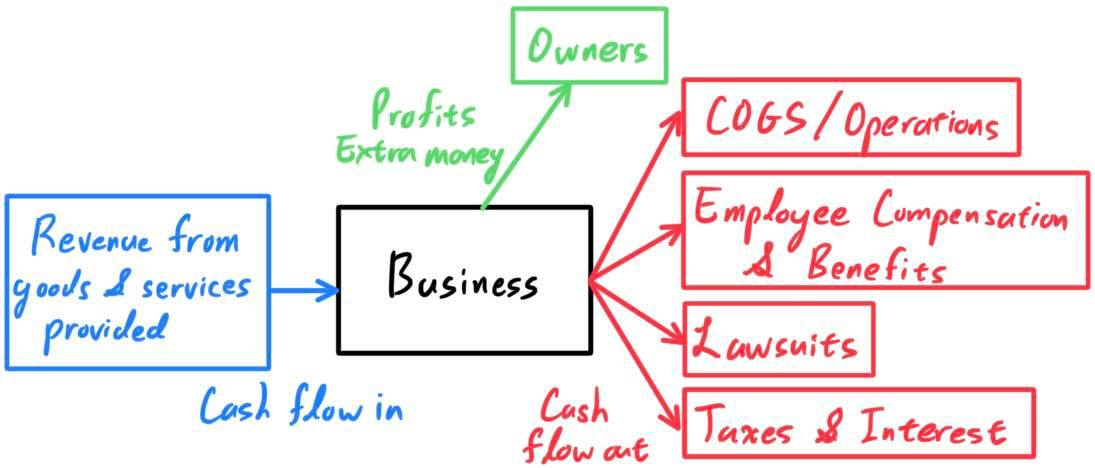
\includegraphics[scale=0.27]{img/Business_Cash_Flow.jpg}
    \end{center}
    Obviously, the owner has a bigger role to play rather than collect profits. They must also decide on things. But since there are usually many owners, these decisions are made through votes in meetings like the annual shareholder meeting. The ownership of a stock really possible rights to earn dividends and possible rights to vote. We will go through the specifics of these powers later. 

    While the most simple model is when all stocks are equal, this is often not the case. Every company's stock structure is different, but as a general guideline I put some examples below. 

    \begin{definition}[Stock Classes and Types]
      Companies may issue different classes of stocks, each with different rights and privileges. 
      \begin{enumerate}
        \item \textbf{Class A shares} may have more voting rights than Class B shares. 
        \item \textbf{Class B shares} may have more dividend rights than Class A shares. 
        \item \textbf{Class C shares} may have more liquidation rights than Class A shares. 
        \item \textbf{Common stocks} are the most common type of stock. Common stock shareholders receive dividends in proportion to the amount of profit generated each year, and they have voting rights. They are usually the lowest priority over a company's income, after the creditors and preferred stock shareholders. 
        \item \textbf{Preferred stock} are much less common and liquid. Preferred stock shareholders receive fixed dividends and no voting rights. They receive payments after bondholders but before common shareholders. 
      \end{enumerate}
    \end{definition}
    
    \begin{definition}[Properties and Powers of Stocks]
      Stocks may also have the following characteristics below. Generally, we work with common and preferred stocks, but other ones may be labeled using letters (e.g. Class A, Class B stocks) that have certain qualities mentioned below. 
      \begin{enumerate}
        \item \textbf{Voting Power}: Nonvoting shares have no voting power while executive shares can be worth 10 votes. 
        \item \textbf{Payment Priority}: Deferred shares are set as a lower priority for dividends and corporate assets. 
        \item \textbf{Cumulative shares} can accumulate dividend payments that have been deferred due to low profits in the past. 
        \item \textbf{Convertible shares} can be converted into different forms of financial assets (e.g. preferred shares may be convertible into common ones, common shares may be convertible into corporate bonds).
      \end{enumerate}
    \end{definition}

  \subsection{Angel Investors and Venture Capital}

    Who would come in an just give you \$10,000 for just some idea? Well this depends mainly on your reputation. If you founded many successful startups with great connections, many investors would be piling up money. However, for most first-time founders, they don't have a name or reputation, which is why they can ask for funding either through competitions (like Y-Combinator) or \textit{angel investors}. Famous founders may skip this outright and get direct funding from institutions, known as \textit{venture capital funding}. 

    \begin{definition}[Angel Investor]
      An \textbf{angel investor} is a high-net-worth individual who provides (non-leveraged) financial backing for small startups or entrepreneurs, typically in exchange for ownership equity or convertible debt. Angel investing is often the primary source of funding for many startups, and it fosters innovation in startups. However, these types of investments are risky and usually do not represent more than 10\% of the angel investor's portfolio. 

      Angel investors usually provide more favorable terms compared to other lenders, since they usually invest in the entrepreneur starting the business rather than the viability of the business. They are focused on helping startups take their first steps, rather than the possible profit they may get from the business. Essentially, angel investors are the opposite of venture capitalists. A company that needs money for operations but is not yet ready for venture capital will typically seek angel capital. 

      They typically use their own money, unlike venture capitalists who pool money from other investors and place them in a managed fund. Additionally, while angel investors are usually individuals, the entity that actually provides the funds may be a LLC, a business, a trust, or an investment fund. 

      The effective internal rate of return for a successful portfolio for angel investors is approximately 22\%. Cheaper sources of financing such as banks are not usually available for such business ventures. 
    \end{definition}

    \begin{definition}[Pre-Seed, Seed Funding]
      A \textbf{pre-seed} or \textbf{Angel round} is the earliest infusion of capital by founders, supporters, and angel investors, to build a prototype and discover initial product-market fit. 
    \end{definition}

    Later on, every startup would want a larger-scale and more reputable \textit{institutional funding} from \textit{venture capital firms}. This can be done by selling additional stocks or through additional \textbf{stock issuance}. 

    \begin{definition}[Venture Capital, VC Rounds]
      \textbf{Venture capital (VC)} is a form of private equity financing that is provided by venture capital firms or funds to startups and early-stage companies that have been deemed to have high long-term growth potential (over decades). Venture capital firms or funds invest in these early-stage companies in exchange for equity, or an ownership stake in the hopes that some of the firms will become successful. 

      Generally, a company would gain investments in certain rounds, or waves:
      \begin{enumerate}
        \item The \textbf{seed round} is generally the first formal equity round with an institutional lead. Investors purchase preferred stock at a valuation set by the lead investor or a convertible note. Companies at this stage may or may not have revenues. Note that companies a this stage have yet to meet requirements for quality for bank loans. 
        \item The \textbf{Series A round} is the name typically given to a company's first significant round of venture capital financing. The name refers to the class of preferred stock sold to investors in exchange for their investment. Series A preferred stock is often convertible into common stock in certain cases such as an IPO or sale of the company. 
        
        Series A rounds typically purchase 10\% to 30\% of the company, and the capital raised during a series A is usually intended to capitalize the company for 6 months to 2 years as it develops products, performs initial marketing/branding, etc. 
        
        \textbf{Series B, Series C, etc.} rounds are additional VC financing rounds, and the progression/price of stock at these rounds is an indication that a company is progressing as expected. However, too much money in too many rounds may be seen as a sign of delayed progress.
        \item \textbf{Series A', Series B', etc.} indicate small follow-on rounds that are integrated into the preceding round, generally on the same terms, to raise additional funds. 
        \item \textbf{Series AA, BB, etc. } denotes a new start after a crunchdown or \textbf{downround} (i.e. the company failed to meet growth objectives) and is essentially starting again under the umbrella of a new group of funders. 
        \item Mezzanine finance rounds, bridge loans, and other debt instruments are used to support a company between venture rounds or before its IPO. 
      \end{enumerate}
      Venture capitalists provide this financing in the interest of generating a return through an eventual "exit" event, such as the company selling shares to the public for the first time in an IPO or disposal of shares happening via a merger or sale. 
    \end{definition}

    The whole process of a VC round can be quite important. Let's first go through the relevant parties. On the company side, we have the founders/stakeholders, who introduce the companies to the investors. In the investor side, each round is typically led by a \textbf{lead investor}, who is typically the best known or most aggressive venture capital firm that is participating in the investment or contributing the largest sum of cash. The lead typically oversees most of the negotiation, legal work, due diligence, etc. It may also introduce the company to other investors. The \textbf{co-investors} are other major investors who contribute alongside the lead investor. Finally, the \textbf{piggyback investors}, who are typically angel investors, rich individuals, institutions, and others who contribute money but take a passive role in the investment. Law firms and accountants who are typically retained by all parties to advise, negotiate, and document the transaction. 

    \begin{enumerate}
      \item \textit{Introduction}. Investors and companies seek each other out through formal and informal business networks, personal connections, paid or unpaid finders, researchers and advisers, and the like. Because there are no public exchanges listing their securities, private companies meet venture capital firms and other private equity investors in several ways, such as speed dating for capital. 

      \item \textit{Offering}. The company provides the investment firm a confidential business plan to secure initial interest. 

      \item \textit{Negotiation of Terms}. Non-binding term sheets, letters of intent, and the like are exchanged back and forth as negotiation documents. 

      \item \textit{Signed term sheet}. Once the parties agree on terms, they sign the term sheet as a non-binding expression of commitment in good faith. These sheets may contain some procedural promises of limited (30 to 60-day) duration like confidentiality, exclusivity on the part of the company (the company will not seek funding from other sources), and standstill provisions (e.g. the company will not undertake any major business changes or enter agreements that would make the transaction infeasible). 
      \item \textit{Definitive documents}. The legal papers that document the final transaction are finalized. They generally include: 
      \begin{enumerate}
        \item \textit{Stock purchase agreements}. The primary contract by which investors exchange money for newly minted shares of preferred stock. 
        \item \textit{Buy-sell agreements, co-sale agreements, right of first refusal, etc}. Agreements by which company founders and other owners of common stock agree to limit their individual ability to sell their shares in favor of the new investors. 
        \item \textit{Investor rights agreements}. Covenants the company makes to new investors, generally includes promises with respect to board seats, negative covenants not to obtain additional financing, sell the company, or make other specified business/financial decisions without the investors' approval, and positive covenants such as inspection rights and promises to provide ongoing financial disclosures. 
        \item \textit{Articles of Incorporation}. Formalize issues like authorization and classes of shares and certain investor protections. 
      \end{enumerate}
      Venture investors obtain special privileges that are not granted to holders of common stock. These are embodied in the various transaction documents, but common rights include: 
      \begin{enumerate}
        \item Anti-dilution protection: If the company ever sells a significant amount of stock at a price lower than the investor paid, then to protect investors against stock dilution they are issued additional shares
        \item Guaranteed board seats
        \item Registration rights: The investors have special rights to demand registration of their stock on public exchanges, and to participate in an IPO and subsequent public offerings
        \item Liquidation preferences: In any liquidation event such as a merger or acquisition, the investors get their money back, often with interest and/or at a multiple, before common stock is paid any funds from liquidation.
        \item Dividends that are given before any common stock
      \end{enumerate}

      \item \textit{Due Diligence}. While negotiating the definitive agreements, the investors examine the financial statements and books and records of the company, and all aspects of its operations. They may require changes to be made. This is the investigation or exercise of care that a reasonable business/person is normally expected to take before entering into an agreement or contract with another party. 

      \item \textit{Agreement} Final agreement occurs when the parties execute all of the transaction documents, completing the deal and funding is announced (although there are often rumors and leaks). 

      \item \textit{Closing} Closing occurs when the investors provide the funding and the company provides stock certificates to the investors. Ideally this would be simultaneous, and contemporaneous with the final agreement. However, conventions in the venture community are fairly lax with respect to timing and formality of closing, and generally depend on the goodwill of the parties and their attorneys. 

      \item \textit{Post-closing}. After the closing a few things may occur: 
      \begin{enumerate}
        \item Conversion of convertible notes. 
        \item Securities filing with relevant state/federal regulators. 
        \item Filing of amended Articles of Incorporation
        \item Preparation of closing binder, containing documentation of entire transaction. 
      \end{enumerate}
    \end{enumerate}

    As a startup accumulates funding, this process may happen multiple times, with the company now in multiple hands. Essentially, these fundings would happen only if the companies are in need of money, since the founders would want to keep as much ownership as possible. 

    \begin{figure}[H]
      \centering 
      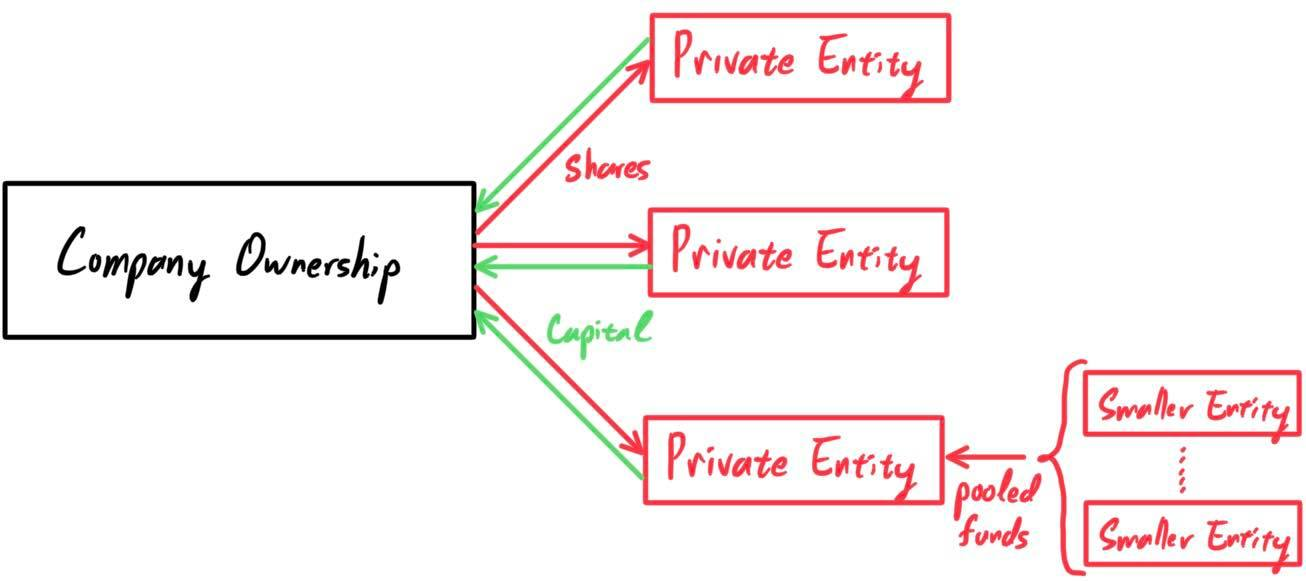
\includegraphics[scale=0.25]{img/company_in_private_hands.jpg}
      \caption{At this point, the ownership of a company is held within the hands of private individuals and firms.} 
      \label{fig:company_in_private_hands}
    \end{figure}

    \begin{example}[Additional Investment]
      Say that you are a founder with 100,000 shares of stock in your company, representing total ownership. 
      \begin{enumerate}
        \item You raise a pre-seed round and give 5000 shares to a family friend, essentially giving her 5\% with anti-dilution protection. She buys it from you at \$2 per share, giving you \$10,000. This sets the valuation of your company at \$200,000. 

        \item Your company does well and has a \textit{minimal viable product}\footnote{This is a popular term in startup culture. } Now you present this to a VC firm for a Series A to raise \$500,000 in the form of 50,000 \textit{additional} shares selling at \$10 each. 

        Firms X, Y, and Z want to invest, with X being the lead investor. X gets 30,000 shares, with Y and Z getting 10,000 each. This is successful, with the valuation of your firm jumping to \$1.5 million. At this point there are a total of 150,000 shares, the family friend has 7500 shares due to the anti-dilution protection (5\%), X has 30,000 (20\%), Y has 10,000 (6.67\%) and Z has 10,000 (6.67\%). You still have 92,500 shares, for a total ownership of 61.67\%. 

        \item You almost have a very good product and need slightly more money, maybe another \$250,000. Therefore, you want to raise a series B with just one VC firm W. However, firms X, Y, Z, not having anti-dilution protection, are pressuring you not to issue more shares. Therefore, you will have to share some of your shares, and you do this by selling 5000 of your own shares at \$50 each. The price is steep, but you are doing very well too. Selling this raises your valuation to $30 \cdot 250,000 = \$7.5$ million. Your ownership decreased to 58.33\%. 
      \end{enumerate}
    \end{example}

    \begin{definition}[Controlling Interest]
      Note that if an entity (individual or organization) has the majority ownership or a \textbf{controlling interest} (at least 50\% in voting rights) of a company, then they have the power to do pretty much whatever they want with the company.
      \footnote{This mainly means common stock, not preferred ones, which generally don't have voting power. }Therefore, the founder must be careful to maintain this majority control. 
    \end{definition}

    \begin{definition}[Proxy Fight]
      One way to gain a controlling interest is through a \textbf{proxy fight}, which is the act of a group of shareholders joining forces and attempting to gather enough shareholder proxy votes to win a corporate vote. This could result in replacing corporate management or the board of directors. 
    \end{definition}

    \begin{definition}[Stock Buyback]
      If the founder wishes, they can always \textbf{buy back} the stock from private investors. This can either be done by negotiating on a price with the private investors or through some predetermined contract.  
    \end{definition}

\section{Accounting} 

  \subsection{Oversight and Regulations}

  \subsection{The Balance Sheet}

    \begin{definition}[Receivables, Payables]
      \textbf{Receivables}, or \textbf{accounts receivable} of a company (the "Company") are debts owed to the Company by its customers for goods or services that have been delivered or used but not yet paid for. 

      \textbf{Payables}, or \textbf{accounts payable} of a company (the "Company") are debts owed to the customers by the Company for goods or services that have been paid for but not yet delivered or used. 
    \end{definition}

    The financial condition of every enterprise can be divided up into its assets and liabilities. The balance sheet provides a snapshot of the assets and liabilities that a company has. 

    \begin{definition}[Assets]
      \textbf{Assets} represent the things that the enterprise has. Some examples of \textbf{current assets} (assets expected to be used through standard business operations within one year) are: 
      \begin{enumerate}
        \item Cash and cash equivalents (cash or highly-liquid assets)
        \item Inventories
        \item
      \end{enumerate}
      Examples of \textbf{non-current assets} (not expected to be used within a year) are: 
      \begin{enumerate}
        \item Property, plant, and equipment (PPE)
        \item Land and real estate
        \item Intangible Assets, such as goodwill, brand recognition, customer loyalty, intellectual property, patents, etc. 
      \end{enumerate}
    \end{definition}

    \begin{definition}[Liabilities]
      \textbf{Liabilities} represent the debts and responsibilities that it needs to pay off. Some examples are: 
      \begin{enumerate}
        \item Accounts payable (liabilities payable to suppliers) 
        \item Salaries payable (future compensation owed to employees)
        \item Deferred revenue (payment by customer that has not yet been earned by the company) 
      \end{enumerate}
      Examples of \textbf{non-current liabilities} are: 
      \begin{enumerate}
          \item 
      \end{enumerate}
    \end{definition}

    \begin{definition}[Shareholder's Equity, or Book Value]
      If the corporation suddenly collapses we can measure how much it is worth by taking its total assets and subtracting from it the total liabilities. The remaining value is called the \textbf{book value} of the company. 
      \[\text{Book Value} = \text{Total Assets} - \text{Total Liabilities}\]
      In other words, if the company were to liquidate all of its assets and pay off all of its liabilities, the amount of money remaining would be the "value" of the company. Since this remaining value would be distributed to the shareholder's of the company (since again, they own the company), this book value is also called the \textbf{shareholder's equity}. 
    \end{definition}

    \begin{definition}[Nominal Value]
      One final characteristic to note is the \textbf{nominal value}, or \textbf{par value}, of a company's stock. Like the face value of a bond when issued, the nominal value of the stock is its stated value. It is an arbitrary value assigned for balance sheet purposes when the company is issuing share capital, and is typically \$1 or less. It has little to no bearing on the stock's market price, so no need to worry about this number.
    \end{definition}

  \subsection{Earnings Sheet}

    Every business's balance sheet can be summarized in terms of the \textbf{Accounting Equation}:

    \begin{equation}
      \text{Total Assets } = \text{ Liabilities } + \text{ Equity}
    \end{equation}

    \textbf{Assets} represent the resources controlled by the company, and the \textbf{liabilities} represent the debts that it owes to creditors. \textbf{Equity} represents the value that would be returned to a company's shareholders if all of the assets were liquidated and all of the company's debts were paid off, also known as the company's \textbf{net assets} or \textbf{book value}. We can also think of equity as representing the shareholders' stake in the company, identified on a company's balance sheet.

    This representation partitions all uses of capital (assets) to the two main sources of capital: debt capital (gotten through lending) and equity capital (gotten through selling shares). For a company keeping accurate accounts, every business transaction will be represented in at least two of its accounts. For instance, if a business takes a loan from a bank, the borrowed money will be reflected in its balance sheet as both an increase in the company's assets and an increase in its loan liability. If a business buys raw materials and pays in cash, it will result in an increase in the company's inventory (an asset) while reducing cash capital (another asset). Because there are two or more accounts affected by every transaction carried out by a company, the accounting system is referred to as \textbf{double-entry accounting}. Here are some of the major components of each part of the balance sheet. Different companies use different terminology, which may be confusing, so we list as many as possible.

    \begin{definition}[Current Assets]
      \begin{enumerate}
        \item \textbf{Cash \& Cash Equivalents} are assets that are cash or can be converted into cash immediately. These include bank accounts and marketable securities, which are debt securities with maturities of less than 90 days. Often times, cash equivalents do not include equity or stock holdings because they can fluctuate in value. Other examples include commercial paper, Treasury bills, and short-term government bonds with maturity dates of 3 months or less. \textbf{Restricted cash} is cash set aside for a particular purpose (e.g. purchasing something or repaying a loan).
        \item \textbf{Marketable Securities} can be included as a separate line (e.g. Apple). They are liquid (maturity of less than 1 year) financial securities that can be quickly converted into cash at a reasonable price, and the rates at which they can be bought or sold have little effect on prices.
        \item \textbf{Inventory} refers to the raw materials used in production, the work-in-progress, and the finished goods produced that are available for sale. The \textit{turnover of inventory} is very important for the company's revenue.
        \item \textbf{Account/Trade Receivables} is the balance of money due to a firm for goods or services delivered or used but not yet paid for by customers. It typically ranges from a few days to a year.
        \item \textbf{Non Trade Receivables} are also receivables due to firm but for something \textit{other} than its normal customer services and goods. They are not related directly to the core operating business of the company. Examples include amounts owed to a company by its employees for loans or wage advances, tax refunds, or insurance claims. They are usually classified as a current assets since they are typically paid within one year.

        Apple has \textbf{vendor non trade receiveables}, which are receivables from its manufacturing vendors resulting from the sale of raw material components to these vendors who manufacture sub-assemblies or assemble final products for the company. Apple purchases these raw material components directly from suppliers.
        \item \textbf{Digital assets} refer to cryptocurrency and assets that can be stored in a blockchain (e.g. smart contracts, NFTs).
        \item \textbf{Operating lease vehicles} (Tesla) refers to the inventory of vehicles that are to be leased out to customers. "Vehicles that are leased as part of our direct vehicle leasing program are classified as operating lease vehicles at cost less accumulated depreciation."
        \item \textbf{Prepaid expenses} is an asset that results from a busness making advance payments for goods or services to be received in the future. They are initially recorded as assets, but their value is expensed over time onto the income statement. For example, assume ABC Company purchases insurance for the upcoming 12 month period. It pays USD120,000 upfront for the insurance policy. ABC Company will initially book the full USD120,000 as a debit to prepaid insurance, an asset on the balance sheet, and a credit to cash. Each month, an adjusting entry will be made to expense USD10,000 (1/12 of the prepaid amount) to the income statement through a credit to prepaid insurance and a debit to insurance expense. In the 12th month, the final USD10,000 will be fully expensed and the prepaid account will be zero.
      \end{enumerate}
    \end{definition}

    \begin{definition}[Noncurrent/Fixed Assets]
      \begin{enumerate}
        \item \textbf{Marketable securities} are explained above, but with a maturity date of longer than 1-year.
        \item \textbf{Property, Plant, and Equipment}
        \item \textbf{Nonoperating Assets} refer to assets that are not essential to the ongoing operations of a business but may still generate income or provide a return on investment (ROI). This is in contrast to \textbf{operating assets}.
        \item \textbf{Intangible assets} are assets that are not physical in nature, which as \textbf{goodwill}, \textbf{brand recognition}, and \textbf{intellectual property}, such as patents, trademarks, and copyrights.
        \item The IFRS16 (2019 lease accounting rule) also stated that when a leasor leases to a lessee, the lessee has to record the leased assets as a \textbf{right-of-use asset}.
      \end{enumerate}
    \end{definition}

    \begin{definition}[Liabilities]
      \begin{enumerate}
        \item \textbf{Accounts/Salaries Payable}
        \item \textbf{Accrued Expenses}
        \item \textbf{Current Maturities on Debt Liabilities}
        \item \textbf{Mortgages, Bonds}
      \end{enumerate}
    \end{definition}

    \begin{definition}[Working Capital]
      Finally, we will use the term \textbf{working capital}, which is really just the \textit{current} assets minus \textit{current} liabilities:
      \begin{equation}
        \text{Working Capital } = \frac{\text{Current Assets}}{\text{Current Liabilities}}
      \end{equation}
    \end{definition}

    When talking about income, we will refer to these terms below many times, which should all be self-explanatory:
    \begin{enumerate}
      \item \textbf{Operating Expenses (OPEX)}: Expenses needed to operate/maintain the business (sometimes synonymous with SG\&A). In the broader sense, we can think of it as: COGS + SG\&A + R\&D + D\&A
      \item \textbf{Cost of Goods Sold (COGS)}: The direct costs associated with producing goods (e.g. direct materials, direct labor, equipment costs, overhead costs for facility).
      \item \textbf{Selling, General \& Administrative Expenses (SG\&A)}: Typically costs associated with a company's overall overhead. It can be thought of as all non-COGS operational expenses. (e.g. accounting, legal, corporate office overhead, advertising, marketing, rent)
      \item \textbf{Research \& Development (R\&D)}: Reseach \& Development (which are tax-deductible)
      \item \textbf{Depreciation \& Amortization (D\&A)}: The depreciation of CAPEX assets are accounted for in here.
      \item \textbf{Capital Expenditures (CAPEX)}: Purchases that a business makes as an investment (e.g. real estate, factory, computers, furniture, intellectual property, copyrights, patents) to help it generate more revenue. CAPEX purchases are not immediately reported on an income statement. Rather, it is treated as an asset on the balance sheet, that is deducted over the course of several years as a depreciation expense in D\&A. Ideally, the increase in revenue made from this CAPEX investment would outweigh the depreciation rate of the investment.
      \item \textbf{Revenue}:  Total Worth of a company's goods \& services sold
      \item \textbf{Gross Profit}: Revenue - COGS
      \item \textbf{EBITDA}: Gross Profit - SG\&A - R\&D
      \item \textbf{Operating Income/EBIT}: Revenue - OPEX
      \item \textbf{Net Income}: Operating Income - Taxes - Interest Expenses on Debts
    \end{enumerate}

  \subsection{Cash Flow Statement}

  \subsection{Ratio Measures}

    A quick and easy way to measure the health of a company is by looking at its financial ratios. They compare two quantities of a certain company and are usually good indicators of different states of a business. Note that \textbf{earnings per share (EPS)} refers to the total net income divided by the shares outstanding, representing the amount of earnings one shareholder would have.

    \begin{enumerate}
      \item \textbf{Working Capital ratio} is similar to working capital, but we divide the current assets by the current liabilities to compare the two:
      \begin{equation}
        \text{Working Capital } = \frac{\text{Current Assets}}{\text{Current Liabilities}}
      \end{equation}

      \item The \textbf{Price to Earnings (P/E) ratio} measures the market cap of the company relative to its total net income. In here, we are comparing the market value of the company with the company's ability to generate money. If the ratio is too high, then this may indicate that the market value is too high relative to the amount of profit the company is making, meaning that the company may be overvalued.
      \begin{equation}
        P/E = \frac{\text{Market Cap}}{\text{Net Income}} = \frac{\text{Stock Price}}{\text{EPS}}
      \end{equation}
      There are actually many different types of P/E ratios, which are all worth mentioning here:
      \begin{enumerate}
        \item The regular P/E ratio is also called a \textbf{trailing PE ratio} because it is based on the previous periods of earnings, usually the \textbf{last twelve months (LTM)}.
        \item Investors often also use the \textbf{\textit{forward} P/E ratio}, which uses the \textit{expected} future earnings (EPS). This is reasonable since the stock-market is always forward-looking.
        \item The \textbf{Shiller P/E ratio} is a trailing ratio but rather than looking at LTM, which may flucuate based on market/seasonal conditions, it looks at the earnings of the past 10-years.
      \end{enumerate}

      \item The \textbf{Price to Book (P/B) ratio} measures the market cap of the company relative to the book value. Therefore, this is a comparison between the believed and actual value of the business. It is almost always the case where this ratio is above $1.0$, but occasionally it falls below. If it is below $1$, then this means that if the company liquidated all of its assets and sold everything, we would earn more money than we paid for. This is a signal of undervalued companies. However, dim future prospects, poor management, forseeable regulatory measures, etc. could drive this ratio down, also signaling a terrible company to invest in.
      \begin{equation}
        P/B = \frac{\text{Market Cap}}{\text{Book Value}}
      \end{equation}

      \item The \textbf{current ratio} measures the \textit{current} assets to \textit{current} liabilities of a firm. This essentially measures the firm's liquidity, i.e. whether it has enough resources (current assets) to pay its current liabilities. It calculates how many dollars in current assets are available for each dollar in short-term debt.
      \begin{equation}
        \text{Current Ratio} = \frac{\text{Current Assets}}{\text{Current Liabilities}}
      \end{equation}

      \item The \textbf{quick ratio} is a more conservative view of the current ratio, as it now excludes inventory (which is considered a part of current assets).
      \begin{equation}
        \text{Quick Ratio} = \frac{\text{Current Assets } - \text{ Inventories}}{\text{Current Liabilities}}
      \end{equation}

      \item The \textbf{Debt to Equity ratio}, also called the \textbf{acid test}, measures the \textit{total} liabilities relative to the \textit{total} equity. It measures the ability of the company to use its current assets to retire current liabilities. It provides an indication of how the firm finances its assest. A high ratio indicates that the company is financing a large percentage of its assets with debt, not a good thing.
      \begin{equation}
        \text{D/E } = \frac{\text{Total Liabilities}}{\text{Total Equity}}
      \end{equation}

      \item The \textbf{Return on Equity (ROE)} measures profitability and how effectively a company uses shareholder money to make a profit, usually as a percentage \%. It compares the amount of profits generated based on the amount of equity lent out for funding. If the net income was okay but the total equity was extremely large, then this means that the company used a lot of equity to generate this okay profit; so the company did \textit{not} efficiently use shareholder money.
      \begin{equation}
        \text{ROE } = \frac{\text{Net Income}}{\text{Total Equity}}
      \end{equation}
    \end{enumerate}

    Now, we present data on these ratios by sectors. The U.S. \textbf{Securities and Exchange Commission}, known as the \textbf{SEC}, has been created through the Securities Exchange Act of 1934 to help restore investor confidence following the stock market crash of 1929. The SEC is an independent government agency tasked with protecting investors, maintaining a fair and orderly market, and facilitating capital formation. SEC filings are regulatory documents required of all public companies to provide key information to investors and potential investors.

    The annual and quarterly reports are the most important filings of the SEC since they contain the financial statements of the company (balance sheet, income statement, and cash flow statement). Note that these statements are not unique to public companies; private companies also have these statements, so knowledge about them would help for all types of businesses.

  \subsection{Current Reports}

\section{Corporate Structure}

  \subsection{Management Hierarchy}

    There is a difference between \textit{ownership} and \textit{management} of a company. Before the 20th century, many companies were small, family-owned, and family-run. However, many are large international conglomerates that trade publicly on multiple exchanges. 

    In order to create a corporation in which stockholders' interest are looked after, many firms have implemented a two-tier \textbf{corporate hierarchy}, or a \textbf{chain of command}. The most common corporate structure in the U.S. consists of a board of directors and a management team. Generally, the management looks after the day-to-day operations, and the board ensures that the shareholders are adequately represented. 

    Note that an individual may be only in the board, only in the management team, or in both. In fact, many boards include current and past members of the management team, including the CEO, the CFO, the COO, along with the retired CEO, family members, etc. Generally, the hierarchy is divided into the following groups: 
    \begin{enumerate}
      \item Board of directors, with the chairman at the top
      \item C-Suite Executive officers
      \item Vice presidents, directors 
      \item Management of smaller departments
      \item Employees
    \end{enumerate}

    \begin{definition}[Board of Directors]
      The \textbf{board of directors} are elected by the shareholders. Every member in the board falls into one of three categories: 
      \begin{enumerate}
        \item The \textbf{board chair} is technically the leader of the corporation and is responsible for running the board smoothly and effectively. Their duties include
        \begin{enumerate}
          \item maintaining strong communication with the CEO and high-level executives
          \item formulating the company's business strategy
          \item representing management and the board to the general public and shareholders
          \item maintaining corporate integrity
        \end{enumerate}
        The chair is elected from the board of directors. 

        \item \textbf{Inside directors} are chosen from within the company and are individuals that work in the company daily. They are responsible for
        \begin{enumerate}
          \item approving high-level budgets prepared by upper-management
          \item implementing and monitoring business strategy
          \item approving core corporate initiatives and projects
        \end{enumerate}
        Inside directors are either shareholders or high-level managers from within the company. 

        \item \textbf{Outside directors} have the same responsibilities as the inside directors in determining strategic direction and corporate policy. However, they are chosen externally and are considered independent of the company. Their purpose is to provide unbiased perspectives on issues brought to the board. 
      \end{enumerate}
    \end{definition}

    \begin{definition}[Management Team]
      The \textbf{management team} is directly responsible for the company's day-to-day operations and profitability. The \textbf{C-Suite} refers to the group of a corporation's top senior executives, with positions all starting with the letter 'C' for 'Chief.'
      \begin{enumerate}
        \item The \textbf{chief executive officer (CEO)} is typically responsible for the corporation's entire operations and is the main liaison between the board of directors and corporate operations. It is the CEO's responsibility to implement board decisions and initiatives, as well as the maintain the smooth operation of the firm with senior management's assistance. 
        
        Because the board is in charge of executive functions, and the CEO is responsible for integrating company policy into day-to-day operations, the CEO often fills the role of the board chair. 
        \item The \textbf{chief operations officer (COO)} is responsible for the corporation's operations and looks after issues related to marketing, sales, production, and personnel. The COO is often more hands-on than the CEO. 
        \item The \textbf{chief financial officer (CFO)} is responsible for analyzing and reviewing financial data, reporting financial performance, preparing budgets, and monitoring expenditures and costs. The CFO is required to present this information to the board and to the SEC. 
        \item The \textbf{chief risk officer (CRO)} is an executive in charge of managing risks to the company, including complying with government regulations, managing investments, guarding intellectual property, and others. 
        \item The \textbf{chief information officer (CIO)} is the company executive responsible for the management, implementation, and usability of information and computer technologies. 
        \item The \textbf{chief technology officer (CTO)} is the executive in charge of an organization's technological needs as well as its R\&D. 
      \end{enumerate}
      An \textbf{interim} position refers to a person appointed by a company's board of directors to assume a certain role during a time of transition of as the result of the sudden departure of the company's previous individual.
    \end{definition}

    \begin{definition}[President]
      The role of \textbf{president} is quite loose and can be used differently depending on the corporation. The president is generally referred to as the leader of a company's executive group. Generally, the board of directors sets the policy, the president executes the policy and reports back to the board, and then the board reports back to the shareholders, the ultimate owners. 
      \begin{enumerate}
          \item The president is the leader of a segment or a critical part of the overall company (rather than the leader of the overall company). 
          \item In smaller businesses, the president may be the CEO or may even be the owner of the company. 
          \item The president often holds the position of the COO, since they lead the day-to-day operations. The president has several vice presidents for different parts of the company reporting to them.\footnote{Note that the CEO is not always the chair of the board, and the president is not always the COO. }
      \end{enumerate}
    \end{definition}

  \subsection{Sectors and Industries}

    \begin{definition}[Consumer Staples]
      
    \end{definition}

    \begin{definition}[Consumer Discretionary]
      
    \end{definition}

    \begin{definition}[Information Technology]
      
    \end{definition}

    \begin{definition}[Finance]
      
    \end{definition}

    \begin{definition}[Utilities]
      
    \end{definition}

    \begin{definition}[Energy]
      
    \end{definition}

  \subsection{Business Models}

    \begin{definition}[Retailer]
      
    \end{definition}

    \begin{definition}[Wholesaler]
      
    \end{definition}

    \begin{definition}[Subscription]
      
    \end{definition}

    \begin{example}[Apple]
    
    \end{example}

    \begin{example}[Costco]
      
    \end{example}

  \subsection{Departments}

    Now we get into more specific details of the company structure. 

    \begin{definition}[Human Resources (HR)]
      
    \end{definition}

    \begin{definition}[Sales \& Marketing]
      
    \end{definition}

    \begin{definition}[Information Technology (IT)]
      
    \end{definition}

    \begin{definition}[Research and Development (R\&D)]
      
    \end{definition}

    \begin{definition}[Operations]
      
    \end{definition}

  \subsection{Lifecycle}


  \subsection{Expansion and Integration}

    Companies can expand in multiple ways, including M\&As, etc. We will elaborate more on this. 

    \begin{definition}[Value Chain]
      A \textbf{value chain} is a step-by-step business model that describes the full range of activities needed to create a product or service. For companies that produce goods, a value chain comprises the steps that involve bringing a product from conception to distribution, and everything in between, such as procuring raw materials, manufacturing functions, and marketing activities. 

      A company can conduct \textbf{value-chain analysis} by evaluating the detailed procedures involved in each step of its business: that is, to maximize value at each specific point in a firm's processes. The purpose of a value-chain analysis is to increase production efficiency while minimizing costs. 
    \end{definition}

    \begin{definition}[Distribution Model]
      A \textbf{distribution model}, or \textbf{distribution channel}, is the manner in which goods move from the manufacturer to the outlet where the consumer purchases them. The conventional distribution model has three levels:
      \begin{equation}
        \text{Producer } \implies \text{ Wholesaler } \implies \text{ Retailer}
      \end{equation}
      There are many ways a business can construct a distribution model, which may get much more complicated. 
    \end{definition}

    \begin{definition}[Vertical Integration]
      \textbf{Vertical integration} is a strategy whereby a company owns or controls its suppliers, distributors, or retail locations to control its value of supply chain. Vertical integration benefits companies by allowing them to control processes, reduce costs, and improve efficiencies. However, it has its disadvantages, including the significant amounts of capital investment required. 
      \begin{enumerate}
        \item \textbf{Backward integration} is when a company expands backward on the production path into manufacturing, meaning a retailer buys the manufacturer of the product. 
        \item \textbf{Forward integration} is when a company expands by purchasing and controlling the direct distribution of supply of its products. This cuts out the middleman and increases profits. For example, a clothing manufacturer can open its own retail location to sell its products. 
      \end{enumerate}
    \end{definition}

    \begin{example}[Netflix]
      Netflix started as a DVD rental business before moving into online streaming of films and movies licensed from major studios. Then, Netflix executives realized they could improve their margins by producing their own original content. Now, Netflix uses its distribution model to promote its original content. 
    \end{example}

    \begin{definition}[Horizontal Integration]
      \textbf{Horizontal integration} is the acquisition of a business operating at the same level of the value chain in the same industry. This is in contrast to vertical integration, where firms expand into upstream or downstream activities, which are at different stages of production. 

      The advantages of horizontal integration include creating economies of scale and reducing competition. However, this can lead to oligopolies or even monopolies, which is why horizontal mergers are heavily scrutinized under antitrust laws. 
    \end{definition}

    \begin{example}[Disney, Pixar]
      Disney's 2006 acquisition of Pixar in the entertainment media industry is an example of horizontal integration. 
    \end{example}

\section{Public Investment}

  \subsection{Initial Public Offerings}

    Perhaps after a few years, the firm has grown to the point where funding on an even larger scale to support even more expansion is needed. Private sources may be too restrictive or small, and so companies may need to tap into the capital of the general public. Thus, they can do a \textbf{public offering}, an issuance of the stock to the general public rather than private entities. This process of an \textbf{initial public offering (IPO)} and the company being listed on a stock exchange is what is referred to as a company "going public." 

    \begin{figure}[H]
      \centering 
      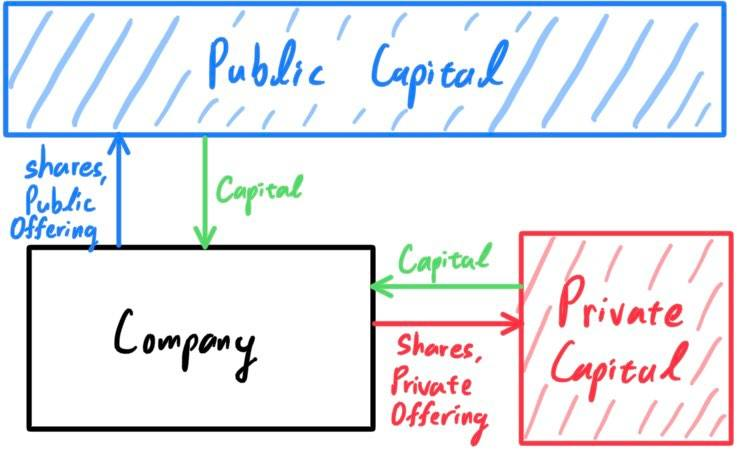
\includegraphics[scale=0.27]{img/Going_public.jpg}
      \caption{Companies would like to access public capital in addition to private capital since it is much larger. } 
      \label{fig:going_public}
    \end{figure}

    While the idea is simple, it is hard to pull off efficiently. This requires great technical knowledge of finance and a thorough understanding of the valuation of the firm. This combination of expertise and navigating regulatory requirements are best done by an investment bank. 

    \begin{definition}[Investment Banks]
      \textbf{Investment banks} advise businesses and governments on how to meet their financial challenges. They offer the following services. 
      \begin{enumerate}
        \item \textit{Underwriting. }The bank can recommend the best way to raise funds, whether it be by selling an ownership stake in the company through a stock offer or borrowing from the public through a bond issue. IBs can help determine how to price these instruments by utilizing sophisticated financial models. 
        \item \textit{Valuation. }In a stock offering, financial analysts will look at factors, e.g. earnings potential and management team strength, to estimate how much a share of a company is worth. In a bond offering, the bank will look at prevailing interest rates for similarly rated businesses to figure out how much it will have to compensate borrowers. 
        \item \textit{Mergers \& Acquisitions. }IBs can offer advice in a Merger and Acquisition (M\&A) scenario. They can advise its management team on how much the company is worth and how to structure M\&A deals. 
        \item \textit{Due Diligence. }They must create the documentation that must go to the SEC before the company can sell shares. This means compiling financial statements and other documents. 
      \end{enumerate}
    \end{definition}

    \begin{definition}[Underwriters]
      An \textbf{underwriting group} is a temporary association of investment bankers and broker-dealers who wish to purchase a new issue of securities from an issuer in order to distribute the issue to investors at a profit.\footnote{In reality, the task of underwriting securities often falls on more than one bank. In larger offerings, the managing underwriter will often form a \textbf{syndicate} (temporary alliance of businesses that manages a large transaction) of other banks that sell a portion of the shares. } The underwriting group shares the risk and aids in the successful distribution of the new securities issue once the issuance goes public. 
      \begin{enumerate}
        \item The group buys the issuance (of new stocks/bonds) from the firm first at a specified price and then sells it to the public, as opposed to the company selling the shares directly to investors. 
        \item The underwriting group resells the issues to investors in order to make a profit. The profit is referred to as the \textbf{underwriting spread}. 
      \end{enumerate}
      For the issuing company, having an underwriting group means that they are paid upfront for the shares they are issuing. As a result, a significant amount of risk is removed from the issuing company and taken on by the underwriting group. The issuing company no longer has to sell the inventory of its stock directly to investors. The profit or loss for the group is determined by how the new stock performs on the market. 

      The underwriter has two options for distributing shares to initial investors: 
      \begin{enumerate}
        \item \textbf{Book-building}, in which shares can be awarded to investors of their choosing. (Usually this happens) 
        \item \textbf{Auctions}, in which investors who are willing to bid above the offer price receive the shares. (Rare, but a notable example is Google's 2004 IPO)
      \end{enumerate}
      The commission fee per share ranges anywhere from 3\% to 7\%, which may be worth having the safety and expertise of underwriters. 
    \end{definition}

    \begin{figure}[H]
      \centering 
      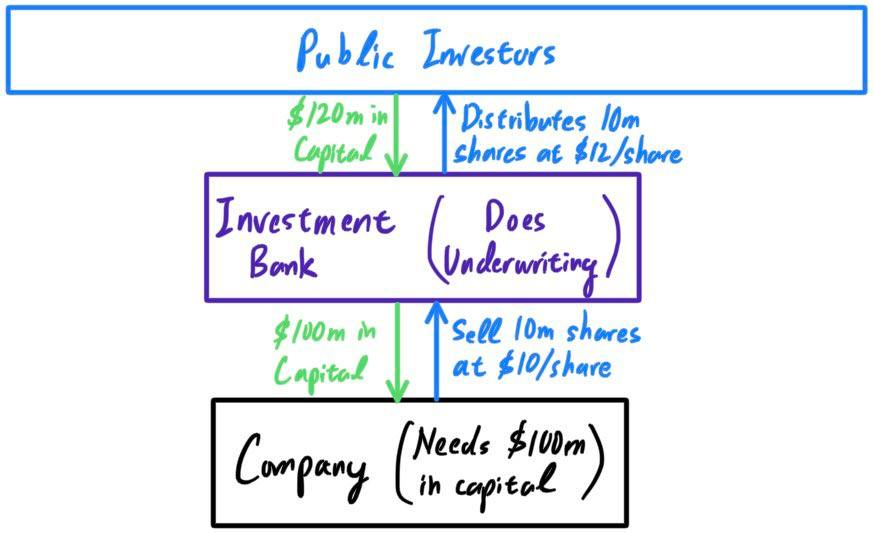
\includegraphics[scale=0.27]{img/Investment_bank_underwriting.jpg}
      \caption{Investment banks, through underwriting services, facilitate public offerings.} 
      \label{fig:investment_bank_underwriting}
    \end{figure}

    \begin{example}[IPO of Water Filtering Company]
      Suppose Acme Water Filter Company hopes to obtain \$1 million in an initial public offering. Based on a variety of factors, including the firm’s expected earnings over the next few years, Federici Investment Bankers determines that investors will be willing to pay \$11 each for 100,000 shares of the company’s stock. As the sole underwriter of the issue, Federici buys all the shares at \$10 apiece from Acme. If it manages to sell all 100,000 at \$11, the bank makes a nice \$100,000 profit (100,000 shares x \$1 spread). 

      However, depending on its arrangement with the issuer, Federici may be on the hook if the public’s appetite is weaker than expected. If it has to lower the price to an average of \$9 a share to liquidate its holdings, it’s lost \$100,000. Therefore, pricing securities can be tricky. Investment banks generally have to outbid other institutions who also want to handle the transaction on behalf of the issuer. But if their spread isn’t big enough, they won’t be able to squeeze a healthy return out of the sale. 
    \end{example}

    \begin{definition}[Types of Circulating Stocks]
      With these, we can organize the number of stocks circulating in different levels, from biggest to smallest:
      \begin{enumerate}
        \item \textbf{Authorized shares} refers to the maximum number of shares that a corporation is legally permitted to issue. Companies don't usually get close to this number due to market conditions, which will be explained later. 
        \item \textbf{Shares issued} refers to the total number of shares issued, including all public shares, private shares, and treasury shares. 
        \item \textbf{Outstanding shares} refer to a company's stock currently held by all shareholders, both public and private shares (including RSUs). It does not include treasury stocks however. 
        \item \textbf{Floating shares} are the shares considered available for the general public. Moreover, the floating percentage represents the portion of outstanding shares that are floating: 
        \begin{equation}
          \text{Floating Percentage} = \frac{\text{Floating Shares}}{\text{Shares Outstanding}}
        \end{equation}
      \end{enumerate}
      \begin{center}
        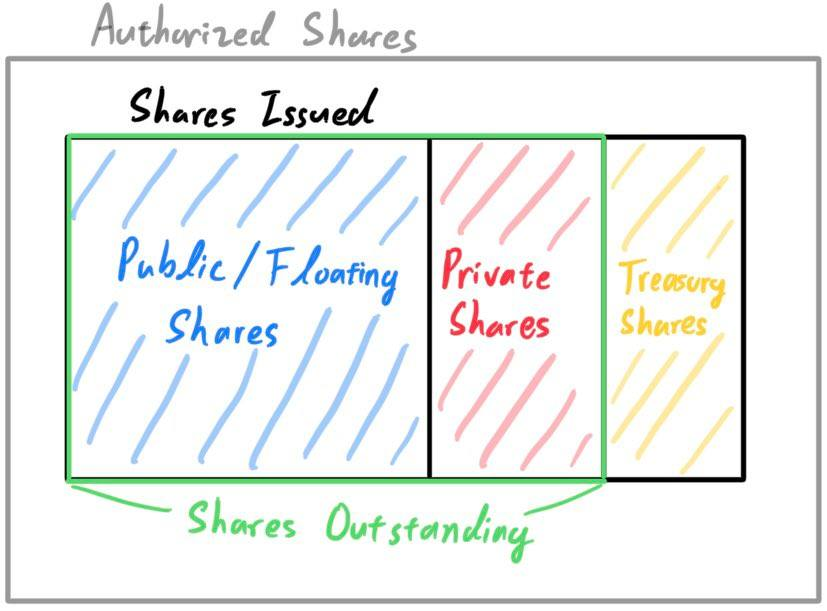
\includegraphics[scale=0.25]{img/Shares_Outstanding.jpg}
      \end{center}
    \end{definition}

    \begin{definition}[Stock Splits]
      Later on, \textbf{stock splits} can be done to increase liquidity if the stock price is too high or for other reasons. \textbf{Reverse stock splits} may also be done. 
    \end{definition}

  \subsection{Direct Listings}

    \begin{definition}[Direct Listing]
      Companies that can't afford underwriting or don't want share dilution choose the \textbf{direct listing} (aka. Direct Placement or Direct Public Offerings) process rather than an IPO. Without an intermediary, however, there is no safety net ensuring the shares sell. In a direct listing, no new shares are created and only existing, outstanding shares are sold with no underwriters involved. 
    \end{definition}

  \subsection{SPACs}

    \begin{definition}[Shell Company]
      A \textbf{shell company} is a company that exists only on paper and has no significant assets or operations. 
    \end{definition}

  \subsection{Seasoned Issue}

  \subsection{Rights Offerings}

    \begin{definition}[Rights Offering]
      A \textbf{rights offering (issue)} permits companies to raise additional equity through the primary market after already having securities enter the secondary market. Current investors are offered prorated (distributed) rights based on the shares they currently own, and others can invest anew in newly minted shares.
    \end{definition}

\section{Corporate Restructuring}

  \subsection{Private Equity}

    Rather than going from private to public. There may be times where a company needs to go from public to private, i.e. the shareholders are no longer able to trade them in the public market. This can be because the public's opinion of a company's value is much more noisy, resulting in more emotional distress in investors, employees, and management. Another reason is that for companies that may need to undergo major changes, a temporary central authority may be needed. The three most common types of going private transactions are: 
    \begin{enumerate}
      \item private equity leveraged buyouts
      \item management buyouts
      \item tender offers
    \end{enumerate}

    We explain all of them here. 

    \begin{definition}[Private Equity]
      \textbf{Private Equity} is an alternative investment class that consists of capital that is not listed on a public exchange. It is composed of funds and investors that directly invest in private companies. Private equity investment comes primarily from institutional and accredited investors, who can dedicate substantial sums of money for extended time periods. The process for investment is as such: 
      \begin{enumerate}
        \item A \textbf{private equity firm}, also known as the \textbf{general partner (GP)}, gathers investors, known as the \textbf{limited partners (LP)}, who would like to invest. 
        \item The firm then invests it in some private business or other investment vehicle. This investment is known as the \textbf{private equity fund}. 
        \item Note that the private equity fund is really owned by the limited partners, but it managed by the general partner. In fact, the LP typically own 99\% of shares in the fund, while the GP owns 1\%. 
        \item Unlike public investments, holding periods for private equity investments last much longer, usually 10+ years. This is to ensure a turnaround for distressed companies or to enable liquidity events such as an IPO or sale to a public company.  
      \end{enumerate}
    \end{definition}

    Some advantages and disadvantages of private equity include: 
    \begin{enumerate}
      \item Advantage: It is favored by companies because it allows them access to liquidity as an alternative to conventional financial mechanisms, such as high interest bank loans or listing on public markets. 
      \item Advantage: For private companies, private equity financing can help them attempt unorthodox growth strategies away from the glare of public markets. 
      \item Advantage: The pressure of quarterly earnings dramatically reduces the time frame available to senior management to turn a company around or experiment with new ways to cut losses or make money. 
      \item Disadvantage: It can be difficult to liquidate holdings in private equity because, unlike public markets, a ready-made order book that matches buyers with sellers is not available. A firm has to undertake a search for a buyer in order to make a sale of its investment. 
      \item Disadvantage: Pricing of shares for a company in private equity is determined through negotiations between buyers and sellers and not by market forces. 
      \item Disadvantage: The rights of private equity shareholders are generally decided on a case-by-case basis through negotiations instead of a broad governance framework. 
    \end{enumerate}

    \begin{definition}[Buyout]
      A \textbf{buyout} is the acquisition of a controlling interest in a company. That is, the company's shares are bought by an entity to gain a controlling interest in that company.  
      \begin{enumerate}
        \item If the stake is bought by the firm's management, it is known as a \textbf{management buyout (MBO)}.

        \item A \textbf{friendly buyout/takeover} is a scenario in which a target company is willingly acquired by another company. Such action is subject to approval by both the target company's shareholders and the U.S. Department of Justice. In situations where the DOJ fails to grant approval, it's typically because the deal violates antitrust (anti-monopoly) laws. 
        
        In a friendly takeover, a public offer of stock/cash is made by the acquiring firm. The board of the target firm will publicly approve the buyout terms, which must then be approved by shareholders (this is usually not a problem is the board agrees to it) and regulators. The acquiring company usually strives to extend fair buyout terms, offering to buy shares at a premium to the current market price.

        \item A \textbf{hostile takeover} is when the target company is unwillingly acquired by another company. This is accomplished by directly going to the company's shareholders or fighting to replace management to get the acquisition approved. It can be done through either a tender offer or a proxy fight. 
      \end{enumerate}
    \end{definition}

    \begin{definition}[Leveraged Buyouts]
      Many buyouts are performed as \textbf{leveraged buyouts (LBOs)}. Usually, the acquiring company may not want to commit too much capital to buy the target company. So, the acquiring company partners up with a private equity firm, which raises funds that covers 50\% to 90\% of the total cost. These funds can come in multiple ways: 
      \begin{enumerate}
        \item Bank Financing: The sponsor uses borrowed funds from a bank or a group of banks, called a syndicate. 
        \item Private Placement of Bonds: Bonds are offered through a private placement (an offering of debt instruments to pre-selected investors). Investors pay cash upfront for the face value of the bond and in return, get paid, an interest rate until the maturity date of the bond. 
        \item Subordinated/Mezzanine Debt: This is a method of obtaining funding without offering collateral, but often requires a higher interest rate or other benefits. 
      \end{enumerate}
      The private equity sponsor loans these funds to the acquiring company (with an interest rate, of course), the acquiring company buys the target company, and the acquisition is complete. 

      Notice that this is a high-risk high-reward strategy, where the acquisition has to realize high returns and cash flows in order to pay the interest on the debt. The target company's assets are typically provided as collateral for the debt, and buyout firms sometimes sell parts of the target company to pay down the debt. In come cases, the acquiring company is also provided as additional collateral. Therefore, in the case where the acquiring company defaults, the private equity firm would get the target company and possibly the acquiring company. 

      Firms that specialize in funding and facilitating buyouts (\textbf{buyout firms}), act alone or together on deals, and are usually financed by institutional investors, wealthy individuals, or loans. 
    \end{definition}

    \begin{definition}[Tender Offer]
      A \textbf{tender offer} occurs when a company or individual makes a public offer to buy most or all of a company's shares. This is another type of buyout and may or may not be leveraged. 

      Sometimes, tender offers are made (and accepted) even when the current management team of the target company does not want the company to be sold. In this situation, this would be a hostile takeover. 
    \end{definition}

  \subsection{Mergers and Acquisitions}

    In M\&As, it is either company A acquires company B, or A and B merge as equals. When company A acquires company B, company A is called the \textit{parent company} while company B is called the \textit{subsidiary}. 

    \begin{definition}[Spinoff]
      Rather than performing a buyout on an independent company, the company can \textit{create} a new independent company through a \textbf{spinoff}, which is the creation of an independent company through the sale or distribution of new shares of a parent company. 

      The spin off will have a separate management structure and a new name, but it will retain the same assets, intellectual property, and human resources. Spinoffs may occur for many reasons, such as allocation of resources or a divergence of plans. 
    \end{definition}

    \begin{definition}[Parent Company]
      A parent company holds a controlling stake (at least 50\%) of its subsidiaries, giving it control of its operations. Parent companies can be either hands-on or hands-off owners of its subsidiaries, depending on the amount of managerial control given to subsidiary managers, but will always maintain a certain level of active control. There are some types of parent companies:
      \begin{enumerate}
        \item A \textbf{conglomerate} is a corporation that is made up of a number of different, sometimes unrelated businesses. In a conglomerate, one parent company owns a controlling stake in a number of smaller companies all of whom conduct businesses separately and independently. 
        
        Conglomerates allows businesses to diversify their portfolio, but the large size of conglomerates can actually hurt the value of their stock (known as the \textit{conglomerate discount}). The financial health of a conglomerate can be difficult to discern by investors sine the management is too complicated. 
        \item A \textbf{holding company}, or an \textbf{umbrella company}, is a passive business entity that doesn't manufacture anything, sell any products or service, or conduct any other business operations. Rather, holding companies only hold the controlling stock in other companies. It may oversee the company's management decisions, it does not actively participate in running a business's day-to-day operations. Holding companies are protected from losses accrued by subsidiaries and receive tax benefits.
      \end{enumerate}
      Because parent companies own more than 50\% of the voting stock in a subsidiary, they have to produce financial statements that combine the parent and subsidiary financial statements into one larger set of financial statements. 
    \end{definition}

    \begin{example}[Berkshire Hathaway]
      Warren Buffet's Berkshire Hathaway is a conglomerate having a majority stake in over 50 companies as well as minority holdings in dozens more companies. It successfully manages companies involved in everything from plane manufacturing and textiles to insurance and real estate. 
    \end{example}

    \begin{example}[General Electric]
      General Electric (GE), originally an electronics company and innovation lab, the company has expanded to own firms working in energy, real estate, finance, media, and healthcare. 
    \end{example}

    \begin{definition}[Subsidiary]
      The \textbf{subsidiary} is the company that is owned, with a controlling interest, by a parent company. If a subsidiary is 100\% owned by another firm, the subsidiary is referred to as a \textbf{wholly owned subsidiary}. 
    \end{definition}

    \begin{example}[Alphabet]
      Alphabet is one of the world's largest technology conglomerates, with a market capitalization of \$1.4 trillion as of Feburary, 2021. Its flagship subsidiary is Google, but owns other companies such as
      \begin{enumerate}
        \item Nest: sells smart-home products
        \item DoubleClick: ad management and ad serving solutions
        \item Looker: business intelligence software and data analytics
        \item Youtube: online video-sharing platform
        \item Waze: mobile navigation app
        \item Fitbit Inc.: wearable fitness devices and app
      \end{enumerate}
    \end{example}

  \subsection{Sister and Parent Companies}


  \subsection{Shell Companies}


  \subsection{Bankruptcy}

    Different types, such as liquidation or restructuring. 

\section{Company Valuation}

  \subsection{Discounted Cash Flow}

  \subsection{Comparables}

\section{Primary Debt Markets}

    \begin{definition}[Bond]
      \textbf{Bonds} are units of corporate debt issued by companies and securitized as tradeable assets. It is a \textbf{fixed income instrument} since bonds are traditionally paid a fixed interest rate (coupon) to debtholders). 

      When investors buy bonds, they essentially lend bond issuers money. In return, bond issuers agree to pay investors interest on bonds through the life of the bond and to repay the face value of bonds upon maturity. They initial price of most bonds is typically set \textbf{at par} (meaning set at nominal, or face value), usually \$100 or \$1000 face value per individual bond. A bond has the following components
      \begin{enumerate}
        \item the \textbf{face value}, which is the money amount the bond will be worth at maturity
        \item the \textbf{coupon rate}, i.e. the rate of interest the bond issuer will pay on the face value of the bond, e.g. a rate of 5\%. We can view the coupon rate as 
        \[\text{Coupon Rate} = \frac{\text{Annual Coupon Payment}}{\text{Bond Face Value}}\]
        \item \textbf{coupon dates}, which are the dates on which the bond issuer will make interest payments. Payments can be made in any interval, but the standard is in semiannual payments. 
        \item the \textbf{maturity date}, which is when the bond will mature and the bond issuer will pay the bondholder the face value of the bond 
        \item the \textbf{issue price}, which is the price at which the bond issuer originally sells the bonds
      \end{enumerate}
      When an investor buys a bond at face value of \$1000 from a corporation/government at a semiannual interest rate of 3\% with a maturity date of 30 years, then every 6 months, the bondholder will receive \$30 for 30 years. After the 30 years, the bond will mature and the investor will receive the face value of the bond back. Therefore, the bondholder will have \$2,800. 
    \end{definition}

    \begin{definition}[Types of Bonds by Issuer] 
      There are four primary categories of bonds sold in the markets, excluding foreign bonds. 
      \begin{enumerate}
        \item \textbf{Corporate bonds} are issued by companies. Companies issue bonds rather than seek bank loans for debt financing in many cases because bond markets offer more favorable terms and lower interest rates.
        \item \textbf{Municipal bonds} are issued by states and municipalities (local governments). Some municipal bonds offer tax-free coupon income for investors. 
        \item \textbf{Government bonds}, or sometimes called \textbf{treasuries}, are issued by the U.S. Treasury. Government bonds issued by national governments may be referred to as sovereign debt. 
        \begin{enumerate}
            \item Those with a year or less to maturity are called \textbf{Bills}
            \item Those with 1-10 years to maturity are called \textbf{Notes}
            \item Those with more than 10 years to maturity are called \textbf{Bonds}
        \end{enumerate}
        \item \textbf{Agency bonds} are those issued by government-affiliated organizations (such as Fannie Mae or Freddie Mac). 
      \end{enumerate}
    \end{definition}

    \begin{definition}[Types of Bonds by Grade]
      Bonds can also be categorized by their credit ratings. 
      \begin{enumerate}
        \item \textbf{Investment-grade bonds} are those rated BBB or higher by Standard \& Poor's or Baa3 or higher by Moody's. 
        \item \textbf{High-yield bonds} are those rated below investment grade (BB+ or lower by Standard \& Poor's or Ba1 or lower by Moody's). 
        \item \textbf{Junk bonds} are those rated below investment grade. 
      \end{enumerate}
    \end{definition}

    \begin{definition}[Extra Properties of Bonds]
      The bonds available for investors come in different varieties, separated by the rate or type of interest or coupon payment, being recalled by the issuer, or other attributes. 
      \begin{enumerate}
        \item \textbf{Zero-coupon bonds} do not pay coupon payments and instead are issued at a discount to their par value that will generate a return once the bondholder is paid the full face value when the bond matures. U.S. Treasury bills are a zero-coupon bond. 
        \item \textbf{Convertible bonds} are debt instruments with an option that allows bondholders to convert their debt into stock (equity) at some point, depending on certain conditions like the share price. 
        
        For example, imagine a company that needs to borrow \$1 million to fund a new project. They could borrow by issuing bonds with a 12\% coupon that matures in 10 years. However, if they knew that there were some investors willing to buy bonds with an 8\% coupon that allowed them to convert the bond into stock if the stock’s price rose above a certain value, they might prefer to issue those. The convertible bond may be the best solution for the company because they would have lower interest payments while the project was in its early stages. If the investors converted their bonds, the other shareholders would be diluted, but the company would not have to pay any more interest or the principal of the bond. 
        
        \item \textbf{Reverse convertible bonds} are like convertible bonds, but now the power to convert debts into stock lies in the hands of the bond issuers. Issuers generally exercise the reverse convertible bond's option if the underlying shares have fallen below a set price, often referred to as the knock-in level, in which case the bondholders will receive the stock rather than the principal and any additional coupons. Their yields are generally higher, though. 
        
        Say XYZ bank issues a reverse convertible bond on the bank's own debt with a built-in put option on the shares of ABC Corp., a blue chip company. The bond may have a stated yield of 10\% to 20\%, but if the shares in ABC decrease substantially in value, the bank holds the right to issue the blue-chip shares to the bondholder, instead of paying cash at the bond's maturity.
        
        \item \textbf{Callable bonds} is one that can be "called" back by the company before it matures. 
        
        Assume that a company has borrowed \$1 million by issuing bonds with a 10\% coupon that mature in 10 years. If interest rates decline (or the company’s credit rating improves) in year 5 when the company could borrow for 8\%, they will call or buy the bonds back from the bondholders for the principal amount and reissue new bonds at a lower coupon rate. 
        
        \item \textbf{Puttable bonds} allows the bondholders to put or sell the bond back to the company before it has matured. This is valuable for investors who are worried that a bond may fall in value, or if they think interest rates will rise and they want to get their principal back before the bond falls in value.
      \end{enumerate}
    \end{definition}

  \subsection{Interest Rates}

  \subsection{Treasury Auctions}

    \begin{definition}[Treasury Bonds]
      \textbf{Treasury bonds} are issued by the U.S. government and are considered to be the safest bonds available. 
      \begin{enumerate}
        \item The \textbf{Treasury bill} is a short-term debt obligation backed by the U.S. government with a maturity of less than one year. 
        \item The \textbf{Treasury note} is a marketable U.S. government debt security with a fixed interest rate and a maturity between one and 10 years.
        \item The \textbf{10-year Treasury bond} is a bond issued by the U.S. Treasury that matures in 10 years. 
        \item The \textbf{30-year Treasury bond} is a bond issued by the U.S. Treasury that matures in 30 years. 
        \item The \textbf{Treasury Inflation-Protected Securities (TIPS)} is a bond issued by the U.S. Treasury that is indexed to inflation to protect investors from the negative effects of inflation. 
      \end{enumerate}
    \end{definition}

    Treasury bills, notes, and bonds are issued through an electronic bill Dutch auction.\footnote{The website for upcoming auctions can be found \href{https://www.treasurydirect.gov/auctions/upcoming/}{here}.} A \textbf{Dutch auction} is an auction in which the price of something offered is determined after taking in all bids to arrive at the highest price at which the total offering can be sold. The bond auction is open to the public, both institutional and individual investors. 24 \textbf{primary dealers} (financial institutions and brokerages) are required to participate. It is divided into competitive and noncompetitive bids.
    \begin{itemize}
        \item \textbf{Competitive bids} are bids where the buyer specifies the rate that they will accept. It is mainly submitted by institutional investors, and competitive bidding is limited to 35\% of the offering amount for each bidder.
        \item \textbf{Noncompetitive bidding} are bids where the buyer agrees to accept the rate determined at the auction (same rate as that determined by competitive bids). It is submitted often by individuals, and noncompetitive bidding is limited to \$5 million per auction.
    \end{itemize}

    \begin{example}[Dutch Auction for Treasury Bonds]
      It is best to explain through an example: Suppose the Treasury seeks to raise \$9 million in two-year notes with a 5\% coupon. Entities can bid up to 30 days in advance of the auction, and let us assume that the submitted bids are as follows:
      \begin{itemize}
          \item \$1 million at 4.79\%
          \item \$2.5 million at 4.85\%
          \item \$2 million at 4.96\%
          \item \$1.5 million at 5\%
          \item \$3 million at 5.07\%
          \item \$1 million at 5.1\%
          \item \$5 million at 5.5\%
      \end{itemize}
      The bids with the lowest yield will be accepted first since the issuer will prefer to pay lower yields to its bond investors. In this case, since the Treasury is looking to raise \$9 million, it will accept the bids with the lowest yield up to 5.07\%. At this mark, only \$2 million of the \$3 million bid will be approved. All bids above the 5.07\% yield will be rejected, and bids below will be accepted. This auction is cleared at 5.07\%, and all successful bidders receive the 5.07\% yield.
    \end{example}

    \begin{definition}[Zero Coupon Bonds]
      \textbf{Zero-coupon bonds} do not pay coupon payments and are instead issued at a discount to their par value that will generate a return once the bondholder is paid the full face value when the bond matures (e.g., U.S. Treasury bills).
    \end{definition}

    \begin{definition}[Zero Coupon Bond]
      A \textbf{zero coupon bond (ZCB)} with maturity $T$ is an asset that pays $1$ at time $T$ (and nothing else). 
    \end{definition}

    Let $V(t, T)$ be value at current time $t$ of a ZCB with maturity $T$, for $t \leq T$. Then, it must be the case that $V(T, T) = 1$. Accounting for interest rates and the discounted value of money, we get the following result. 

    \subsubsection{Daycount Conventions}

      Another important concept to mention is the daycount conventions in the financial markets. Note that since a year consists of 365 days, when doing discrete compounding we cannot easily calculate $r/m$. For example, if we wanted to do quarterly payments, we would have $m = 4$ but we cannot split 365 into 4 parts. Note the following days in each quarter. 

      \begin{table}[H]
        \centering
        \caption{Number of days between quarterly dates}
        \label{table:quarterly_days}
        \begin{tabular}{@{}lc@{}}
        \hline
        Period                               & Days \\ 
        \hline
        16 March 2011 to 16 June 2011        & 92   \\
        16 June 2011 to 16 September 2011    & 92   \\
        16 September 2011 to 16 December 2011& 91   \\
        16 December 2011 to 16 March 2012    & 91   \\ 
        \hline
        \end{tabular}
      \end{table}
      
      There are lots of imperfections and therefore there are many different market conventions. We list some of them. 

      \begin{definition}[Act/365]
        The \textbf{actual 365} (act 365) daycount convention calculates the quarterly interest rate by dividing by the number of days by 365. 
      \end{definition}

      \begin{definition}[Act/360]
        The \textbf{actual 360} (act/360) daycount convention calculates the quaterly interest by dividing the number of days by 360. 
      \end{definition}

      \begin{definition}[Act/Act]
        The \textbf{actual actual} (act/act) convention calculates the quaterly interest by dividing by the actual number of days in each year. This accounts for leap years. 
      \end{definition}    

      \begin{definition}[30/360]
        The \textbf{30 360} (30/360) convention assumes that there are 30 days in each month and was designed to produce equal amounts of interest payment each month or quarter. It calculates the quarterly interest by simply $120/360 = 1/4$.
      \end{definition}

      \begin{example}[Accural Factors for Each Quarter]
        The \textbf{accural factor} is the convention to divide a year into equal time periods, denoted by $\alpha$. For each quarter above, we can get 
      \end{example}

  \subsection{Corporate Debt}

\section{Bond Valuation}

    \begin{theorem}[Value of Zero Coupon Bond]
      The value of a zero coupon bond at time $t$ with maturity $T$ with continuously compounded interest rate is 
      \begin{equation}
        V(t, T) = e^{-r(T-t)}
      \end{equation}
      and with discretely compounded interest rate is 
      \begin{equation}
        V(t, T) = \frac{1}{(1 + r_A)^{T - t}}
      \end{equation}
      where $r_A$ is the annually compounded rate. 
    \end{theorem}
    \begin{proof}
      We prove this result by \textit{discounting cashflows back to today}, which means to take whatever cashflow in the future, and discounting it at the interest rate to current time. If you had $e^{-r (T - t)}$ at time $t$, then you can invest it at the interest rate $r$, compounded continuously, to get 
      \begin{equation}
        e^{- r(T - t)} \cdot e^{r (T - t)} = 1
      \end{equation}
      after time $T - t$, which is what the ZCB pays. 
    \end{proof}

    If we assume that the price $P$ is a good approximate of the value $V$, then we can substitute it into the equation to get an estimate of the interest rate.  
    \begin{equation}
      P(t, T) (1 + r_A)^{(T - t)} = 1 \text{ or } P(t, T) e^{r (T - t)} = 1
    \end{equation}
    Note that $r$ is not constant across time, so it should really be written as 
    \begin{equation}
      P(t, T) (1 + r_A(t, T))^{(T - t)} = 1 \text{ or } P(t, T) e^{r(t, T) (T - t)} = 1
    \end{equation}

  \subsection{Interest Rates and Inflation}

    Now, we can integrate our knowledge of markets with that of bonds. Let there be entities $E_1, \ldots, E_n$ each owning some arbitrary number of bonds from the federal government, labeled $Fed$. As in all markets, the equilibrium price of certain bonds are determined by shift in supply and demand of the bond.

    Interest rates (the fed funds rate) heavily influence the demand, and therefore the price, of a bond. Recall that the fed funds rates acts as pretty much a "baseline interest rate" for all kinds of debt obligations throughout the nation. Since the option to lend money to the U.S. government (with a pretty much guarantee in payment back) is always available, banks would charge at lower interests to borrow from each other. This effective fed funds rate that banks use when borrowing is now the "minimum" interest rate that they will charge to consumers when lending (since to get profits their interest on lending must be greater than their interest on borrowing).

    To be updated: Describe the process of how the fed funds rate affects the coupon rates in newly issued bonds.
    Let's focus on entities $E_1$ and $E_2$, and say that they each invested $\$10,000$ into $Fed$ to buy $10$ $\$1,000$ 10-year bonds with an annual coupon rate of $10\%$. Therefore, they will receive a fixed-income of $\$100 \times 10 = \$1,000$ per year for the next 10 years. Now, say that the Fed issues $10$ new 10-year $\$1,000$ bonds (with same maturity date). A good thing to keep in mind is that whenever the Fed issues some new bonds, \textit{these new bonds determine the standards for how much fixed-income securities are worth}.

    \begin{enumerate}
      \item If these bonds have a $20\%$ interest rate, this translates to fixed payments of $\$200$ per year. Remember, these are the new standards for bonds now: \textit{Any 10-year fixed-income security that pumps out $\$200$/year is worth $\$1,000$}, according to the Fed. Therefore, with this standard, any 10-year fixed-income security that pumps out $\$100$/year must be worth twice as little: $\$500$. Therefore, this new standard will cause the demand for $\$100$ fixed-income securities to drop to $\$500$.
      \begin{center}
        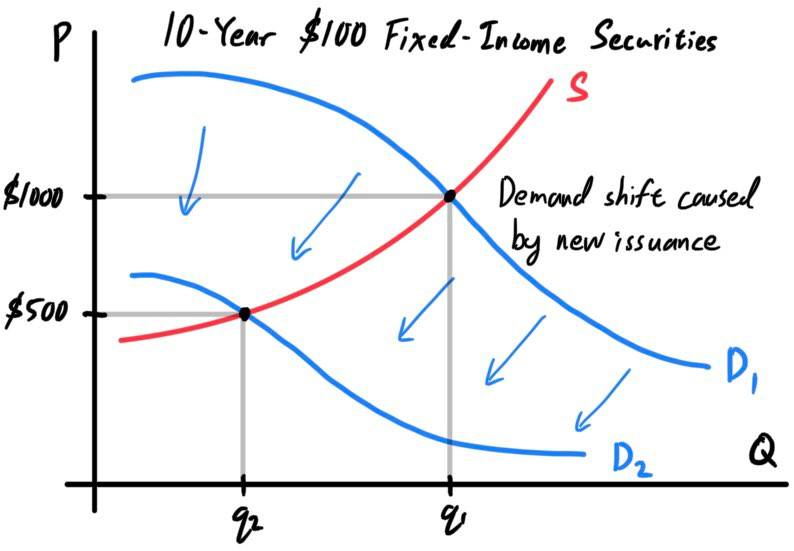
\includegraphics[width=0.4\textwidth]{img/Bond_Demand_Decrease.jpg}
      \end{center}
      \item If these bonds have a $5\%$ interest rate, this translates to fixed payments of $\$50$ per year. So, the new standard for bond is: \textit{Any 10-year fixed-income security that pumps out $\$50$ a year is worth $\$1,000$}. Therefore, with this standard, any 10-year fixed-income security that pumps out $\$100$/year must be worth twice as much: $\$2,000$. Therefore, this new standard will cause the demand for $\$100$ fixed-income securities to rise to $\$2,000$.
      \begin{center}
        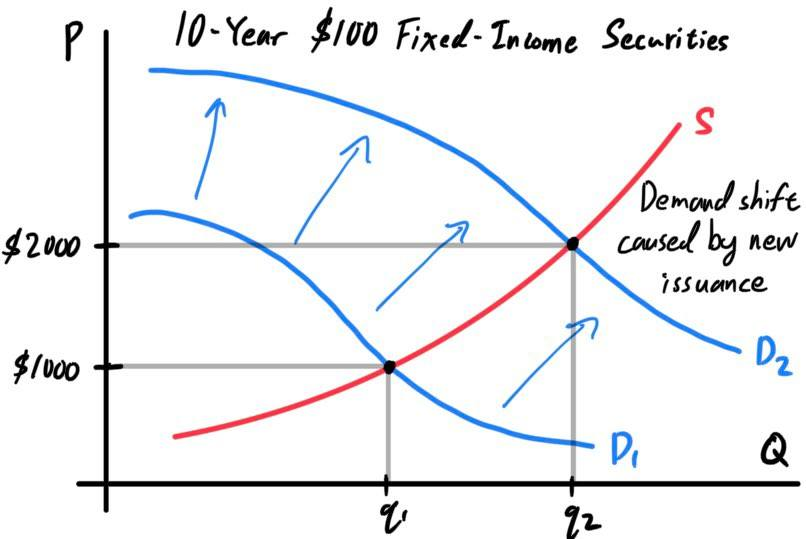
\includegraphics[width=0.4\textwidth]{img/Bond_Demand_Increase.jpg}
      \end{center}
    \end{enumerate}

    The adept reader may notice that the bond market behaves in a such a way that the current interest rates of each bond of the same type (i.e. same issuer and same maturity time: 10-year T-bond) throughout the market equal out.

    \begin{enumerate}
      \item In the first scenario, the market balances out such that buying a 10-year fixed-income security generating $\$100$/year for $\$500$ is the same as buying a 10-year fixed-income security generating $\$200$/year for $\$1,000$.
      \item In the second, the market balances out such that buying a 10-year fixed-income security generating $\$50$/year for $\$1000$ is the same as buying a 10-year fixed-income security generating $\$100$/year for $\$2,000$.
    \end{enumerate}

    Another major influence on bonds (and really any fixed-income instrument) is \textbf{inflation}. Some securities may rise in value along with inflation, and therefore are protected, but bonds have none of this. Therefore, if we expect inflation rates to rise in the next few years, then this will decrease the value and therefore the price of bonds.

  \subsection{Creditworthiness}

    \begin{definition}[Credit Quality]
      \textbf{Credit quality} is a measurement of an individual's or company's creditworthiness, or the ability to repay its debt. It can also be seen as a measure of the level of counterparty risk to the lender/creditor. They are measured by private independent \textbf{credit rating agencies}, the most popular being
      \begin{enumerate}
        \item Standard \& Poor's 
        \item Moody's 
        \item Fitch
      \end{enumerate}
      each with its own designations, ranging from 
      \begin{enumerate}
        \item high \textbf{investment-grade}: AAA to AA
        \item medium \textbf{investment-grade}: A to BBB
        \item low \textbf{junk, high-yield, or subprime}: BB, B, CCC, CC, C
        \item Already in default: D 
      \end{enumerate}
      Credit scores can be assigned to multiple things:
      \begin{enumerate}
        \item \textbf{Bond ratings} are used to determine the risk that the bond issuer will default on its payments. 
        \item \textbf{Corporate credit ratings} are based on a firm's financial statements, including the specific company's capital structure, credit payment history, revenue, and earnings.
        \item \textbf{FICO scores} determine an individual's credit quality for credit card expenses, mortgages, auto loans, etc. It ranges from 300-850. 
      \end{enumerate}
      Investing in securities issued by the U.S. treasury is considered the absolute safest way to invest in bonds, then bluechip corporations, and then smaller companies. 
    \end{definition}

    Note that if a security has a lower credit quality, the risk of default is greater and these securities may have greater potential profits (e.g. pay more interest, better dividends, great potential, etc.) 


  \subsection{Present Value of Future Cash Flows (DCF)}

    When we are valuing a bond, we are basically trying to answer the question: \textit{How much would an investor to pay to purchase a bond (of certain type) today?} We can use \textbf{discounted cash flow (DCF)} analysis for this. To compute this bond value (and the values of most other financial assets), we just have to find out the present value of the future income stream discounted at the \textbf{required rate of return}. Let us have a bond with

    \begin{enumerate}
      \item face value of $F$,
      \item coupon rate that determines the annual interest payments to be $C$,
      \item $N$ years until maturity. Note that we can value bonds that have already given out coupon payments. For example, a 10-year bond that has been issued two years ago will have 8 more coupon payments, but we can interpret this as a 8-year bond with a fixed cash flow with the standard of a current dollar.
      \item a required rate of return of $r$, which is the market interest rate; that is, the interest rate of bonds within the market. In other words, we are assuming that the Fed will consistently issue bonds with interest rate $r$ for the duration until maturity. The option to invest in bonds with interest $r$ is always available to us.
    \end{enumerate}
    Then, the formula for the \textbf{present value} of the bond is
    \begin{align*}
      P & = \left( \frac{C}{1 + r} + \frac{C}{(1+r)^2} + \ldots + \frac{C}{(1+r)^N} \right) + \frac{F}{(1+r)^N} \
      & = \left( \sum_{i=1}^N \frac{C}{(1+r)^i} \right) + \frac{F}{(1+r)^N}
    \end{align*}
    To explain this, note the basic fact that a dollar today is worth \textit{more} than a dollar in the future because we always have the opportunity to invest it. THat is, a cash flow today is more valuable than an identical cash flow in the future because a present flow can be invested immediately and begin earning returns, while a future flow cannot. Therefore, if we receive $C$ dollars in the future, it is the same as if we had received $C_0 = C (1 + r)^{-1}$ dollars today at prevailing interest rates $r$ since by investing this at this interest rate gives us
    \begin{equation}
      C_0 (1+r) = C
    \end{equation}
    dollars in the future. A very closely related term is the \textbf{net present value (NPV)}, which is present value but now takes into account the initial investment costs at year $0$. That is, NPV is detrermined by calculating the costs (negative cash flows) and benefits (positive cash flows) for each period of an investment. Therefore, with a slight modification of the original formula gives
    \begin{align*}
      NPV & = -(\text{Initial Investment}) + \left( \sum_{i=1}^N \frac{C}{(1+r)^i} \right) + \frac{F}{(1+r)^N} \
      & = \sum_{i=0}^N \frac{\text{Year i Total Cash Flow}}{(1 + r)^i}
    \end{align*}
    Note that the initial investment (negative value) is included in Year $0$ total cash flow, and the year $N$ total cash flow contains both the coupon payment and the redemption of the face value.
    For example, suppose that you are an investor who wants to purchase a bond, which is redeemable in 10 years for its face value of $\$1,000$ and pays an annual coupon of $5\%$ on the face value (interest payments of $\$50$ per year)? For multiple prevailing interest rates $r$, we can calculate the present value and the net present value of these investments. Remember, that these rates $r$ represent the absolute guaranteed return on investments, so investing in a fixed-income security with interest rates less than $r$ counts as a \textit{loss} (in present value).
    \begin{enumerate}
      \item If $r = 3\%$, then the value of the bond is
      \begin{equation}
        P = \left( \sum_{i=1}^{10} \frac{50}{(1.03)^i} \right) + \frac{1000}{(1.03)^{10}} = \$1170.60 \implies NPV = \$170.60
      \end{equation}
      We would get a profit from this investment because prevailing rates (i.e. guaranteed rate of return) are much lower than the rate of our investment.

      \item If $r = 4\%$, then the value of the bond is
      \begin{equation}
        P = \left( \sum_{i=1}^{10} \frac{50}{(1.04)^i} \right) + \frac{1000}{(1.04)^{10}} = \$1081.11 \implies NPV = \$81.11
      \end{equation}
      We would get a profit from this investment because prevailing rates are lower than the rate of our investment.

      \item If $r = 5\%$, then the value of the bond is
      \begin{equation}
        P = \left( \sum_{i=1}^{10} \frac{50}{(1.05)^i} \right) + \frac{1000}{(1.05)^{10}} = \$1000 \implies NPV = \$0
      \end{equation}
      We would get nothing from this investment because prevailing rates are equal to the rate of our investment.

      \item If $r = 6\%$, then the value of the bond is
      \begin{equation}
        P = \left( \sum_{i=1}^{10} \frac{50}{(1.06)^i} \right) + \frac{1000}{(1.06)^{10}} = \$926.40 \implies NPV = -\$75.60
      \end{equation}
      We would lose money from this investment because prevailing rates are higher than the rate of our investment.

      \item If $r = 7\%$, then the value of the bond is
      \begin{equation}
        P = \left( \sum_{i=1}^{10} \frac{50}{(1.07)^i} \right) + \frac{1000}{(1.07)^{10}} = \$859.53 \implies NPV = -\$140.47
      \end{equation}
      We would lose money from this investment because prevailing rates are much higher than the rate of our investment.
    \end{enumerate}
    These prevailing interest rate would change as a direct result of the fed funds rate. Note that actual prices of these bonds may fluctuate based on other factors, such as creditworthiness, inflation, foreign exchange, etc.

  \subsection{Current Yield \& Yield to Maturity (YTM)}

    If the current price of a bond is given, together with details of coupon and redemption date, then this information can be used to compute the \textbf{current yield}, which is the percentage return based on the price you have bought it:
    \begin{equation}
      \text{Current Yield } = \frac{\text{Interest Payment}}{\text{Price}}
    \end{equation}

    However, this valuation is limited in multiple ways. First, they don't measure the value of reinvested interest. The \textbf{internal rate of return (IRR)}, or the \textbf{yield to maturity (YTM)}, of an investment in a bond takes this into account (the IRR is a more general term covering other investments, so we will use YTM in this context). Given a bond that is redeemable in $N$ years producing a fixed-income of $C$ (which is the coupon rate time the face value $F$), priced at $P$, the YTM is the value of $r$ satisfying the following equation
    \begin{align*}
      P & = \frac{C}{(1+r)} + \frac{C}{(1+r)^2} + \ldots + \frac{C}{(1+r)^{N}} + \frac{F}{(1+r)^N} \
      & = \left(\sum_{i=1}^N \frac{C}{(1+r)^i} \right) + \frac{F}{(1+r)^N}
    \end{align*}

    What does this YTM actually mean? The IRR (and YTM) of an investment is the rate of return that sets the net present value of all cash flows (both positive and negative) equal to $0$. More colloquially, the YTM tells us what the prevailing interest rate would have to be such that our investment is worth exactly $0$. This process is actually the inverse of what we did last subsection:
    \begin{enumerate}
      \item Previously, we look at the given prevailing interest rates $r$ and compute the value/expected price of a bond.
      \item Here, we look at the price of a bond and determine what prevailing interest rates $r$ would there need to be for us to profit, break even, or lose on this investment.
    \end{enumerate}
    If we expect interest rates on bonds to be higher than the YTM in the future, then we would expect to lose money from this investment if we buy it at a price of $P$. Analogously, if we expect interest rates on bonds to be lower than the YTM, then we would expect to gain money from this investment if we buy it at a price of $P$.
    Quick refresher on \textbf{annualized returns}. If we make an investment of $C$ dollars and get a profit of $P$ dollars after $N$ years, then we can say that we got a total return of $P/C - 1$, represented as a percentage. But if we would like to represent it as a compounded annual return, we can calculate the annualized return of this investment:
    \begin{equation}
      \sqrt[N]{\frac{P}{C}} - 1
    \end{equation}
    Now we can introduce an extremely useful property of the YTM of a bond: \textit{The YTM represents the annualized rate of return of a bond, given that all coupons are reinvested at a yield equal to the YTM, and that the bond is held to maturity. }
    Suppose we have a bond with face value of $\$100$ and coupon rate of $7\%$, implying coupon payments of $\$7$/year, and the bond is reedemable in 5 years. We see that it has a market price of $\$106.62$. We can compute the YTM by computing the $r$ in the equation:
    \begin{equation}
      \$106.62 = \frac{7}{(1+r)} + \frac{7}{(1+r)^2} + \frac{7}{(1+r)^3} + \frac{7}{(1+r)^4} + \frac{107}{(1+r)^5}
    \end{equation}
    We find that $YTM = 5.46\%$. Calculations are not important here since we do it numerically anyways. Remember that this means that within prevailing interest rates of $5.46\%$, this bond would be worth exactly $\$0$. Furthermore, we can also claim that the annualized rate of return of this bond, given that all coupons are reinvested at the same yield, after 5 years is $5.46\%$. To see what this means, follow the steps:
    \begin{enumerate}
      \item In year 0, we have invested $\$106.62$.
      \item In year 1, we receive a coupon payment of $\$7$, which we invest immediately at the rate of $5.46\%$. Over the next 4 years until the bond matures, the $\$7$ compounds to $\$8.66$.
      \item In year 2, we receive a coupon payment of $\$7$, which we invest immediately at the rate of $5.46\%$. Over the next 3 years until the bond matures, the $\$7$ compounds to $\$8.21$.
      \item In year 3, we receive a coupon payment of $\$7$, which we invest immediately at the rate of $5.46\%$. Over the next 2 years until the bond matures, the $\$7$ compounds to $\$7.79$.
      \item In year 4, we receive a coupon payment of $\$7$, which we invest immediately at the rate of $5.46\%$. Over the next 1 year until the bond matures, the $\$7$ compounds to $\$7.38$.
      \item In year 5, we receive a coupon payment of $\$7$ and the face value of $\$100$. The bond matures.
    \end{enumerate}

    Therefore, after 5 years we have
    \begin{equation}
      \$8.66+\$8.21 + \$7.79 + \$7.38 + \$107 = \$139.04
    \end{equation}
    and so our initial investment of $\$106.62$ increased to $\$139.04$, a total return of $30.47\%$. Annualized over 5 years, this is equivalent to an annual return of $5.46\%$ (same as the YTM as we have said), and so rather than treating the bond as a fixed-income instrument, we can interpret it as an investment that compounds.

  \subsection{Annuities}

    \begin{definition}[Annuity]
      An \textbf{annuity} is a series of fixed cashflows $C$ at specified times $T_i$ for $i = 1, 2, \ldots, n$. 
    \end{definition}

    \begin{theorem}[Value of Annuity]
      The value $V$ at current time $t \leq T_1$ of an annuity can be calculated by summing the value of the zero coupon bonds a each expiry date $T_i$. 
      \begin{equation}
        V(t, \mathbf{T}) = C \sum_{i=1}^n Z(t, T_i)
      \end{equation}
    \end{theorem}

\section{Forwards and Futures}

    \begin{definition}[Derivatives]
      A \textbf{derivative} is a financial security with a value that is reliant upon or derived from, an underlying asset or group of assets. The derivative itself is a contract between two or more parties, and the derivative derives its price from fluctuations in the underlying asset. The most common underlying assets for derivatives are: 
      \begin{enumerate}
        \item stocks
        \item bonds
        \item commodities
        \item currencies
        \item interest rates 
        \item market indexes 
      \end{enumerate}
      They can be traded either OTC (between 2 companies privately) or on an exchange.\footnote{OTC derivatives constitute a greater proportion of the derivatives market, but exchange-traded derivatives have many advantages, such as standardization, liquidity, and elimination of default risk. Originally, derivatives were used to ensure balanced exchange rates for goods traded internationally. With the differing values of national currencies, international traders needed a system to account for differences. }
    \end{definition}

    \begin{example}[Apples and Pies] 
      Suppose you have an apple orchard and you make pies. You can sell apples and pies at a fixed price, but you can also sell them at a future price. For example, you can sell apples at a future price of \$1 per apple. 
    \end{example}

    \begin{definition}[Futures]
      \textbf{Futures contracts} are an agreement between two parties for the purchase and delivery of an asset at an agreed upon price at a future date. Futures trade on an exchange, and the parties involved in the futures transaction are \textit{obligated to fulfill} a commitment to buy or sell the underlying asset. This means that the purchase \textit{must} be made, regardless of the current market price at the expiration date. The amount you pay for the actual futures contract is called the \textbf{premium}. 
    \end{definition}

    \begin{definition}[Forwards]
      A \textbf{forwards contract} is a futures contract but it is traded OTC. 
    \end{definition}

    \begin{example}[Crude Oil]
      Say that a trader wants to speculate on the price of crude oil by entering into a futures contract in May with the expectation that the price will be higher by year-end. The December crude oil futures contract is trading at \$50 and the trader locks in the contract.

      Since oil is traded in increments of 1,000 barrels, the investor now has a position worth \$50,000 of crude oil (1,000 x \$50 = \$50,000). However, the trader will only need to pay a fraction of that amount up-front—the initial margin that they deposit with the broker. 

      From May to December, the price of oil fluctuates as does the value of the futures contract. If oil's price gets too volatile, the broker may ask for additional funds to be deposited into the margin account—a \textbf{maintenance margin}.

      In December, the end date of the contract is approaching, which is on the third Friday of the month. The price of crude oil has risen to \$65, and the trader sells the original contract to exit the position. The net difference is cash-settled, and they earn \$15,000, less any fees and commissions from the broker (\$65 - \$50 = \$15 x 1000 = \$15,000). However, if the price oil had fallen to \$40 instead, the investor would have lost \$10,000 (\$40 - \$50 = negative \$10 x 1000 = negative \$10,000).
    \end{example}

    \begin{example}[Oil Forward]
      Say that on Nov. 6, 2019, Company A buys a futures contract for oil at a price of \$62.22 per barrel that expires Dec. 19, 2019. The company does this because it needs oil in December and is concerned that the price will rise before the company needs to buy. Buying an oil futures contract hedges the company's risk because the seller on the other side of the contract is obligated to deliver oil to Company-A for \$62.22 per barrel once the contract has expired. Assume oil prices rise to \$80 per barrel by Dec. 19, 2019. Company-A can accept delivery of the oil from the seller of the futures contract, but if it no longer needs the oil, it can also sell the contract before expiration and keep the profits. 

      In this example, it is possible that both the futures buyer and seller were hedging risk. Company-A needed oil in the future and wanted to offset the risk that the price may rise in December with a long position in an oil futures contract. The seller could be an oil company that was concerned about falling oil prices and wanted to lock in a deal. 

      For example, the futures contract for West Texas Intermediate (WTI) oil trades on the CME represents 1,000 barrels of oil. If the price of oil rose from \$62.22 to \$80 per barrel, the trader with the long position—the buyer—in the futures contract would have profited \$17,780 [$(\$80 - \$62.22) \times 1000 = \$17,780$]. The trader with the short position—the seller—in the contract would have a loss of \$17,780.
    \end{example}

    \begin{example}[Stock Futures]
      Suppose individual A believes that the stock price for AMC Entertainment is going to go up and buys a futures contract of 100 shares for \$3 per share which will expire in a month. He will need to pay a small portion of the contract as an initial payment now, but when a month passes, he pays the total \$300. If the price of AMC is \$7, then he can immediately sell the 100 shares he bought to make a profit of $\$4 \times 100 = \$400$. If the price of AMC is lower, then he has a net loss. 
    \end{example}

  \subsection{Settlement}

    Not all futures contracts are settled at expiration by delivering the underlying asset. Many derivatives are cash-settled, which means that the gain or loss in the trade is simply an accounting cash flow to the trader's brokerage account. 

  \subsection{Delivery}
  

\section{Swaps}

  \begin{definition}[Swap]
    \textbf{Swaps} is a derivative contract through which two parties exchange the cash flows or liabilities from two different financial instruments. One cash flow is generally fixed, while the other is variable and is based on a benchmark interest rate, floating currency exchange rate, or index price. The most common examples of swaps can be about: 
    \begin{enumerate}
      \item interest rates
      \item mortgage bonds 
      \item exchange rates
    \end{enumerate}
    Swaps don't trade on exchanges, and retail investors do not generally engage in swaps. Rather, swaps are over the counter contracts primarily between businesses that are customized to the needs of both parties. 
  \end{definition}

  \begin{example}[Interest Rate Swap]
    A trader might use an interest rate swap to switch from a variable interest rate loan to a fixed interest rate loan, or vice versa. 

    Imagine that Company XYZ has borrowed \$1,000,000 and pays a variable rate of interest on the loan that is currently 6\%. XYZ may be concerned about rising interest rates that will increase the costs of this loan or encounter a lender that is reluctant to extend more credit while the company has this variable rate risk. 

    Assume that XYZ creates a swap with Company QRS, which is willing to exchange the payments owed on the variable rate loan for the payments owed on a fixed rate loan of 7\%. That means that XYZ will pay 7\% to QRS on its \$1,000,000 principal, and QRS will pay XYZ 6\% interest on the same principal. At the beginning of the swap, XYZ will just pay QRS the 1\% difference between the two swap rates.

    If interest rates fall so that the variable rate on the original loan is now 5\%, Company XYZ will have to pay Company QRS the 2\% difference on the loan. If interest rates rise to 8\%, then QRS would have to pay XYZ the 1\% difference between the two swap rates. Regardless of how interest rates change, the swap has achieved XYZ's original objective of turning a variable rate loan into a fixed rate loan.
  \end{example}

  \begin{example}[Forex Swap]
    Imagine a European investor, whose investment accounts are all denominated in euros (EUR). This investor purchases shares of a U.S. company through a U.S. exchange using U.S. dollars (USD). Now the investor is exposed to exchange-rate risk while holding that stock. Exchange-rate risk the threat that the value of the euro will increase in relation to the USD. If the value of the euro rises, any profits the investor realizes upon selling the stock become less valuable when they are converted into euros.

    To hedge this risk, the investor could purchase a currency derivative to lock in a specific exchange rate. This kind of derivative is called a currency future or currency swap. 
  \end{example}

\section{Options}

  \begin{definition}[Options]
    An \textbf{options contract} is similar to a futures contract in that it is an agreement between two parties to buy or sell an asset at a predetermined future date for a specific price. The key difference between options and future is that, with an option, the buyer is not obliged to exercise their agreement to buy or sell. It is an opportunity only, not an obligation. The amount you pay for the actual option contract is called the \textbf{premium}. There are two types of options: 
    \begin{enumerate}
        \item A \textbf{put option} is a contract that gives the right to sell an asset at a specific price. It is typically a bearish bet on the market, since you can sell it at a higher price when the price goes down. 
        \item A \textbf{call option} is a contract that gives the right to buy an asset at a specific price. It is typically a bullish bet on the market, since you can buy it at a lower price when the price goes up. 
    \end{enumerate}
    Note that for stock options, a single contract covers 100 shares of the underlying stock. 
  \end{definition}

  \begin{example}[Company Options]
    Company ABC's shares trade at \$60, and a call writer is looking to sell calls at \$65 with a one-month expiration. If the share price stays below \$65 and the options expire, the call writer keeps the shares and can collect another premium by writing calls again. 

    If the share price appreciates to a price above \$65, referred to as being in-the-money, the buyer calls the shares from the seller, purchasing them at \$65. The call-buyer can also sell the options if purchasing the shares is not the desired outcome.
  \end{example}

  \begin{example}[Stock Put Options]
    If you wanted to buy a put option on Intel stock at a strike price of \$48 per share, expecting the stock to go down in price in six months to sit around at \$45 or \$46, you could make a decent profit by exercising your put option and selling those shares at a higher price if the market price goes down. 
  \end{example}

  \begin{example}[Stock Put Options]
    If an investor owns a put option to sell XYZ at \$100, and XYZ’s price falls to \$80 before the option expires, the investor will gain \$20 per share, minus the cost of the premium. If the price of XYZ is above \$100 at expiration, the option is worthless and the investor loses the premium paid upfront.
  \end{example}

  \begin{example}[Stock Call Options]
    Suppose you buy a call option contract of 100 shares of AMC to be bought at \$3 per share, expiring in 6 months, at a premium of \$100. Within the next 6 months, if the price of \$AMC jumps to \$10, then you can exercise the call option to get 100 AMC shares at \$3 per share, even though the market price is $\$10$ per share. You can immediately sell these shares to get a profit of $\$7 \times 100 = \$700$, minus the premium price of $\$100$, for a final profit of $\$600$. 
  \end{example}

  \begin{example}[Stock Call Options]
    For example, an investor opens a call option to buy stock XYZ at a \$50 strike price sometime within the next three months. The stock is currently trading at \$49. If the stock jumps to \$60, the call buyer can exercise the right to buy the stock at \$50. That buyer can then immediately sell the stock for \$60 for a \$10 profit per share. 
        
    Alternatively, the option buyer can simply sell the call and pocket the profit, since the call option is worth \$10 per share. If the option is trading below \$50 at the time the contract expires, the option is worthless. The call buyer loses the upfront payment for the option, called the premium.
  \end{example}

\section{Other Financial Assets}

  \begin{definition}[Alternative Investment]
    An \textbf{alternative investment} is a financial asset that does not fall into one of the conventional investment categories. Conventional categories include stocks, bonds, and cash. Alternative investments include private equity, venture capital, hedge funds, managed futures, art and antiques, commodities, derivatives contracts, and real estate. 
  \end{definition}

  \subsection{Loan-Backed Securities}

    \begin{definition}[Securitization]
      Assets can be created by pooling individual loans and selling shares in that pool, a process called \textbf{securitization}. Securitization has been applied to mortgages, student loans, credit card loans, and auto loans (up to thousands of them in a single security). But with so many loans packaged together, it can be difficult to assess the true quality of the asset. 
    \end{definition}

    \begin{definition}[MBS]
      \textbf{Mortgage backed securities (MBS)} is an investment similar to a bond that is made up of a bundle of home loans bought from the banks that issued them. Investors in MBS receive periodic payments similar to bond coupon payments. The process is as such: 
      \begin{enumerate}
        \item A bank (the "Bank") pays for an individual's (the "Individual") home and receives regular payments from the Individual as a mortgage with a fixed interest rate. 
        \item The Bank pools together mortgages exclusively, which are debts, and sells them at a discount to be packaged as a mortgage-backed security to an investor (the "Investor"), through possibly a broker. This MBS is a type of collateralized bond. 
        \item The Investor now owns the debt security, and an MBS is as safe as the mortgage loans that back it up. The bank takes no risk nor damages if the Individual defaults, since the situation is essentially equivalent to the Investor paying for the Individual's home. 
      \end{enumerate}
      Essentially, the mortgage-backed security turns the bank into an intermediary between the Individual and the Investor. A bank can grant mortgages to its customers and then sell them at a discount for inclusion in an MBS. The bank records the sale as a plus on its balance sheet and loses nothing if the homebuyer defaults sometime down the road. 

      In order to be sold on the markets today, an MBS must have received one of the two top ratings issued by an accredited credit rating agency. 
    \end{definition}

  \subsection{Funds}

    \begin{definition}[Funds]
      A \textbf{fund} is simply a pool of money that is allocated for a specific purpose. Funds can be established for any purpose whatsoever. We can generally divide funds into three categories: 
      \begin{enumerate}
        \item Individual funds
        \item Investment funds
        \item Government funds
      \end{enumerate}
    \end{definition}

    \subsubsection{Individual Funds}

      \begin{definition}[Emergency Funds]
        \textbf{Emergency funds} are personal savings vehicles created by individuals used to cover period of financial hardships. 
      \end{definition}

      \begin{definition}[College Funds]
        \textbf{College funds} are usually tax-advantaged savings plans set up by families to allocate funds for their children's college expenses. 
      \end{definition}

      \begin{definition}[Trust Funds]
        \textbf{Trust funds} are legal arrangement set up by a \textbf{grantor} who appoints a third-party \textbf{trustee} (usually a trust bank) to administer valuable assets for the benefit of a listed beneficiary for a period of time, after which all or a portion of the funds are released to the beneficiary. 

        The primary motivation for establishing a trust fund is for an individual to create a vehicle that sets terms for the way assets are to be held, gathered, or distributed in the future. Generally, the grantor is creating an arrangement that, for a variety of reasons, is carried out after they are no longer mentally competent or alive. The fund can contain nearly any asset imaginable, such as cash, stocks, bonds, property, etc. 

        Some types of trust funds include: 
        \begin{enumerate}
          \item A \textbf{revocable/living trust} lets a grantor better control assets during the grantor's lifetime. The grantor places assets into a trust that can then transfer to any number of designated beneficiaries after the grantor's death. Living trusts are not made public, meaning an estate is distributed with a high level of privacy. While the grantor is still living and not incapacitated, the trust details can be changed or revoked. 
          \item An \textbf{irrecovable trust} is very difficult to change or revoke, but there can be considerable tax benefits for the grantor to effectively give away control of the assets to the trust funds. 
          \item An \textbf{asset protection trust (APT)} is created to protect a person's assets from claims of future creditors. 
          \item A \textbf{blind trust} is created so the beneficiary is not aware of who holds power of attorney for the trust (generally the trustee). 
        \end{enumerate}
      \end{definition}

      \begin{definition}[Retirement Funds]
        \textbf{Retirement funds} are savings vehicles used by individuals saving for retirement. Retirees receive monthly income or pensions from retirement funds.
      \end{definition}

    \subsubsection{Investment Funds}

      \begin{definition}[Mutual Funds]
        \textbf{Mutual funds} are investment funds managed by professional managers who allocate the funds received from individual investors into stocks, bonds, and/or other assets. These funds are managed through stock picking and market timing (that is, choosing securities to invest in and strategizing when to buy and sell them). This means that maintenance fees can be high. 
      \end{definition}

      \begin{definition}[Mutual Fund Family]
        A \textbf{family of mutual funds} is a group of funds that are marketed under one or more brand names, usually having the same distributor (the company which handles selling and redeeming shares of the fund in transactions with investors). Some examples of fund families and their \textbf{assets under management (AUM)} are: 
        \begin{center}
        \begin{tabular}{r|l|l}
          Fund Family & AUM & Fund Name\\
          \hline
          BlackRock & \$8.676 trillion & iShares\\
          Vanguard & \$7.1 trillion & Vanguard\\
          Fidelity & \$4.9 trillion & Fidelity\\
          State Street Global Advisors (SSGA) & \$3.5 trillion & SPDR\\
          Charles Schwab & \$3.25 trillion & Schwab\\
          Goldman Sachs & \$2.1 trillion & GS\\
          Invesco & \$1.349 trillion & Powershares\\
          Wilshire Associates & \$1 trillion & Wilshire\\
          T. Rowe Price & \$991.1 billion & T. Rowe Price \\
          Morgan Stanley & \$715 billion & MS\\
          AllianceBernstein & \$697 billion & AB \\
          WisdomTree Investments & \$41.8 billion & WisdomTree
        \end{tabular}
        \end{center}
        These companies manage these funds. 
      \end{definition}

      \begin{definition}[Management Expense Ratio]
        The \textbf{management expense ratio (MER)} is a measure of a mutual fund's operating costs relative to assets. It is calculated: 
        \[\text{Expense Ratio} = \frac{\text{Total Fund Costs}}{\text{Total Fund Assets}}\]
        The MER refers to how much of a fund's assets are used towards administrative and other operating expenses. It is important because it lets an investor know how much they are paying in costs by investing in a specific fund and how much their returns will be reduced by. The lower the expense ratio the better because it means that an investor is receiving higher returns on their invested capital. 


        Operating expenses can vary depending on the fund, but the expenses within the fund remain relatively stable. The biggest portion of fund expenses is the fee paid to a fund's investment manager, but other costs include recordkeeping, custodial services, taxes, legal expenses, and accounting/auditing fees. Generally, 
        \begin{enumerate}
            \item Funds investing in large companies should not have an MER over 1\%
            \item Funds investing in smaller companies should not have an MER over 1.25\%
        \end{enumerate}
        Any funds with higher MERs are either really expensive or should have a reason that justify their costs. 
      \end{definition}

      \begin{example}[Vanguard S\&P500 ETF MER]
        The \textit{Vanguard S\&P500 ETF} has one of the lowest expense ratios in the industry at 0.03\% annually; investors are charged just \$3 per year for every \$10,000 invested. The \textit{Fidelity Contrafund} is one of the largest actively managed funds in the marketplace with an expense ratio of 0.86\%, or \$86 per \$10,000 per year. 
      \end{example}

      \begin{example}[MERs of Index vs Active Funds]
        Due to the lower management level of index funds, the expense ratios of index funds would be significantly smaller than those of mutual ones. This is indeed the case. 
        \begin{enumerate}
          \item The \textit{AB Large Cap Growth Fund} is an actively managed fund with a net MER of 0.61\%. It's management fee is 0.50\%, meaning that 0.11\% of the total fund assets goes to non-management expenses. 
          \item The \textit{T. Rowe Price Equity Index 500 Fund} is a passive fund designed to replicate the S\&P500. It's net MER is 0.19\%. It's management fee of 0.06\%, meaning that 0.13\% of the total fund assets goes to non-management expenses. 
        \end{enumerate}
      \end{example}

      \begin{definition}[Money-Market Funds]
        \textbf{Money-market funds} are highly liquid mutual funds purchased to earn interest for investors through short-term interest-bearing securities such as Treasury bills and commercial paper. 
      \end{definition}

      \begin{definition}[Exchange-Traded Funds]
        \textbf{Exchange Traded Funds (ETFs)} are similar to mutual funds but traded on the public exchanges like stocks. 
      \end{definition}

      \begin{example}[S\&P500 Funds]
        There are many funds whose portfolio of stocks are designed to track those of the S\&P 500 due to its popularity as a barometer of U.S. equity markets, including both mutual funds and exchange-traded funds (ETFs). Different fund families offer different funds that mimick the S\&P500 differently. They include: 
        \begin{enumerate}
          \item Fidelity 500 Index Fund (FXAIX)
          \item Schwab S\&P500 Index Fund (SWPPX)
          \item Vanguard 500 Index Fund Investor Shares (VFINX) 
          \item State Street S\&P500 Index Fund Class N (SVSPX)
          \item SPDR S\&P500 ETF (SPY)
        \end{enumerate}
        The SPDR funds are also managed by State Street Global Advisors. 
      \end{example}

      \begin{definition}[Index Funds]
        An \textbf{index fund} is a type of mutual fund or an ETF with a portfolio constructed to match or track the components of a financial market index, such as the S\&P500 Index. It is said to provide broad market exposure, low operating expenses, and low portfolio turnover. Index funds seek to match the risk and return of the market, on the theory that in the long-term, the market will outperform any single investment. The most popular index funds track the S\&P500, and other examples include
        \begin{enumerate}
          \item Vanguard 500, made to track the S\&P500 faithfully, in composition and performance. 
          \item Russell 2000, made up of small-cap company stocks
          \item Wilshire 5000 Total Market Index, the largest U.S. equities index 
          \item MSCI EAFE, consisting of foreign stocks from Europe, Australasia, and the Far East
          \item Bloomberg Barclays U.S. Aggregate Bond Index, which follows the total bond market
          \item Nasdaq Composite, made up of 3000 stocks listed on the Nasdaq exchange
          \item Dow Jones Industrial Average (DJIA) consisting of 30 large-cap companies
        \end{enumerate}
      \end{definition}

      \begin{definition}[Hedge Funds]
        \textbf{Hedge funds} are investment vehicles for high-net-worth individuals or institutions designed to increase the return on investors' pooled funds by incorporating high-risk strategies such as short selling, derivatives, and leverage. A few things to note: 
        \begin{enumerate}
          \item They are more expensive compared to conventional investment funds, and will often restrict investment to high-net-worth or sophisticated investors. 
          \item The number of hedge funds throughout the world had exploded, with approximately 11,000 currently and 5500 in North America. 
          \item Even though they were successful in the 1990s and early 2000s, many have underperformed (especially after fees and taxes). 
          \item They are less liquid, since they require a minimum commitment of 1 year, along with specific time periods when money can be withdrawn (e.g. quarterly or biannually). 
          \item Rather than charging an expense ratio only, hedge funds charge both an expense ratio and a performance fee, known as the \textit{Two and Twenty}: a 2\% asset management fee and then a 20\% cut of any gains generated. 
          \item They have much less regulations than all other funds, so they can do pretty much do what they want as long as they disclose the strategy upfront to investors. 
        \end{enumerate}
        It's ironic because the word "hedging" is actually the practice of attempting to reduce risk, but the goal of most hedge funds is to maximize return on investment. 
      \end{definition}

      \begin{definition}[Government Bond Funds]
        Government bond funds are for investors looking to put their money away in low-risk investments through Treasury securities, such as Treasury bonds, or agency-issued debt. Both alternatives are backed by the U.S. government. 
      \end{definition}

    \subsubsection{Government Funds}

      \begin{definition}[Debt-Service Funds]
      \textbf{Debt-service funds} are allocated to repay the government's debt. 
      \end{definition}

      \begin{definition}[Capital Projects Funds]
      \textbf{Capital projects fund} resources are used to finance the capital projects of a country, such as purchasing, building, or renovating equipment, structures, and other capital assets. 
      \end{definition}

      \begin{definition}[Permanent Funds]
      \textbf{Permanent funds} are investments and other resources that the government is not allowed to cash or spend. However, the government normally has the right to spend any revenue these investments generate on appropriate functions of government.
      \end{definition}

  \subsection{Retirement Plans}

\end{document}
